
\documentclass[review]{elsarticle}
\usepackage{hyperref}
\usepackage[margin=1in]{geometry}
\usepackage{graphicx}
\usepackage{amsmath}
\usepackage{placeins}
\usepackage{comment}
\usepackage{textcomp}
\usepackage{gensymb}
\usepackage{lineno}
\usepackage{color}
\usepackage{cleveref}
\usepackage{multicol}

\usepackage[utf8]{inputenc}
\usepackage[english]{babel}

\usepackage[dvipsnames]{xcolor}

%\journal{Journal of Nuclear Materials}
\bibliographystyle{elsarticle-num}

\begin{document}

\begin{frontmatter}

\title{First-principles-derived transport properties of molten chloride salts }

\author[ncsu]{Kai Duemmler}
\author[inl]{Michael Woods}
\author[inl]{Toni Karlsson}
\author[inl]{Ruchi Gakhar}

\author[ncsu,inl]{Benjamin Beeler\corref{qwe}}
\cortext[qwe]{Corresponding author}
\ead{bwbeeler@ncsu.edu}

\address[ncsu]{North Carolina State University, Raleigh, NC 27695}
\address[inl]{Idaho National Laboratory, Idaho Falls, ID 83415}
\date{\today}

\begin{abstract}
Molten salts have many applications ranging from a heat transfer medium in both generation IV nuclear reactor designs and the solar industry to thermal storage systems. While molten salts show promising properties for these applications, there still exists a knowledge gap for the transport properties of molten salts at elevated temperatures. This work uses \textit{ab initio} Molecular Dynamics to investigate the transport properties of KCl, LiCl, KCl-LiCl eutectic, NaCl, MgCl$_{2}$, and NaCl-MgCl$_2$ eutectic molten salt systems. The properties presented here are the diffusion coefficient, viscosity, and isochoric heat capacity. These properties are compared to experimental data where available and other computational work in cases where no experimental data is available. This is the first work to explore timescales over 100 ps via AIMD for the determination of transport properties in molten salts.
\end{abstract}

\end{frontmatter}

%\begin{multicols}{2}

\section{Introduction}
In recent years, the interest in molten salts has been renewed. Historically, molten salts have been used in many different fields including metal production \cite{Zhu2014, VAHIDI2018178}, catalysis production \cite{JIN20202382, HU20204244}, and pyroprocessing methods to handle spent nuclear fuel \cite{CHOI2015572, osti_22107867}. Presently there is also an interest to use various molten salts for thermal energy storage or as a means of transferring heat in the nuclear or solar industry. Some of the generation four (Gen IV) designs for nuclear power plants include molten salts as either the fuel salt in the case of the liquid-salt-fueled design \cite{doi:10.1080/00295450.2019.1586372} or as a moderator/heat transfer material in the case of the solid-fuel design \cite{doi:10.13182/NSE90-374}. There are a few differences in the molten salts between the two designs; in the liquid fuel design, the fuel material is uranium, plutonium, and/or thorium and this fuel as well as the soluble fission products are dissolved within the salt. The solid fuel design is similar to what is currently implemented in light water reactors in the USA but the heat transfer medium is molten salts rather than water. Regardless of the design, the primary function of the molten salt is to transfer the heat generated by fission from the primary loop into the secondary loop \cite{gakhar2021molten}. Molten salt reactors are attractive designs due to their good neutron economy, the ability for online refueling, the possibility for online processing and fission product removal, and inherent safety features \cite{leblanc2010molten}. Two specific safety features are the little to no required pressurization \cite{leblanc2017integral} and the effective residual heat removal systems \cite{SUN2014149}. The latter is an important lesson learned from the Fukushima-Daichi plant in Japan, where a station blackout and generator failure led to the accumulation of residual heat from the core in a light water reactor. Without a proper residual heat removal system, not only can the core be damaged but there can be a release of radioactive gases \cite{SUN2014149}.
 


Historically, the transport properties of materials are often determined via classical molecular dynamics (MD) or experiments \cite{WANG2014262}. There is a general lack of thermophysical and kinetic properties of molten salts, which is linked to the difficulty of handling molten salts. These salts are very sensitive to oxygen due to their hygroscopic nature and other impurities. Some salts are toxic and all irradiated fuel salts are radioactive and contain a number of fission products. Due to the underlying difficulty of conducting experiments to determine transport properties, they are most commonly calculated via classical MD simulations. 

Molecular dynamics  can be divided into two main categories, classical MD and \textit{ab initio} MD (AIMD). The first is classical in which the internal energies are calculated from a parameterized interatomic potential. These potentials need to be parameterized either by fitting to experimental or density functional data and are typically only valid for the compositions and temperature range for which they were parameterized. The second category is AIMD, also called first principles MD. In this method, energies are directly calculated from the electron interactions and do not need to be parameterized. There are trade-offs for both methods, e.g., in classical MD millions or even billions of atoms can be studied for a time scale reaching nanoseconds, while in AIMD the number of atoms is limited to hundreds or thousands, and a time scale of picoseconds. While AIMD is more computationally expensive it is also more accurate as it calculates its energies from electron interactions, not a fitted set of interactions. AIMD has not been used historically to determine transport properties due to computational limitations, as transport properties require a long time to obtain converged behavior from the Green-Kubo relations \cite{PhysRevA.7.1439}.


Two of the most critical transport properties for molten salts are the diffusion coefficient and the viscosity. The diffusion coefficient quantifies the ability of ions within the salt to move, which can influence charge transport, corrosion processes, etc., while the viscosity describes the liquid internal resistance to flow, which is critical for understanding the pumping of fluids. Another reason that viscosity is important in molten salts is that molten salt applications, such as fuel solvents in molten salt reactors, thermal energy storage, or heat carriers for nuclear or solar power, require the accurate calculation of heat transfer and fluid dynamics.

A common way of determining the diffusion coefficient when Brownian motion is present is to fit a linear function to the mean squared displacement (msd) as the slope is directly proportional to the diffusion coefficient \cite{qian1991single}. This method is often referred to as the Einstein relationship and can be seen in \cref{eq:Einstein},

\begin{equation}
  \label{eq:Einstein}
     D = \frac{1}{6N} \lim_{t\to\infty}\frac{d}{dt}\sum_{i=1}^N \langle |r_i(t) - r_i(0)|^2\rangle
\end{equation}

\noindent where \textit{N} is the number of atoms in the system, \textit{r(t)} and \textit{r(0)} are the position vectors at a given time and a reference time, respectively\cite{CHAKRABORTY2015371}. The other computational method that can be used to calculate the diffusion coefficient is the velocity autocorrelation function \cite{rapaport2004art} which takes the form of a Green-Kubo relation.

The historical experiments conducted before the 1970s have been collected by Janz for the diffusion coefficient of both single and multi-component salt systems with reported errors approaching 50$\%$ \cite{janz_Diffusion,janz_osti}. The methods used during this period include the capillary method\cite{bockris1965self}, chronopotentiometry \cite{chemla1976transport}, rotating disc electrode \cite{kuo1975rotating}, and the potential step cyclic voltammetry method \cite{chemla1976transport}. Molten chloride salts have also been studied computationally through classical MD. A common interatomic potential formalism used for molten salts is the Born-Mayer-Huggins potential which has been parametrized and used to study quaternary (Li, Na, K, Cs)Cl and (Li, K, Rb, Cs)Cl \cite{sun2018investigation}, LiCl-KCl \cite{caccamo1980molten,WANG2014262,Bengston2014}, and KCl-MgCl$_2$ \cite{lu2021thermal}, to name a few.


%Viscosity is a transport property that is important for molten salts for various reasons. In general, viscosity is a measurement of a liquid internal resistance to flow \cite{Viswanath2007}. 

Two different kinds of viscosity are measured: dynamic and kinematic viscosity. The dynamic viscosity is the measure of the tangential force per unit area needed to allow one layer to slide against a different layer with a fixed unit distance. The kinematic viscosity requires the density of the liquid to be known, as in \cref{eq:Kinematic_viscosity}, which shows that it is related to dynamic viscosity ($\eta$) through the density ($\rho$) \cite{Viswanath2007}. 

\begin{equation}
  \label{eq:Kinematic_viscosity}
     \nu = \frac{\eta}{\rho}
\end{equation}

 There are various ways to calculate the dynamic viscosity experimentally, including the oscillating-cylinder method, capillary method, and oscillating-cup method \cite{Viswanath2007}. Along with the experimental methods, it is also possible to extract the viscosity of a liquid through computational methods via molecular dynamics in both classical and \textit{ab initio} methods. Two approaches can be used to extract the viscosity of a liquid. The first is to use the Stokes-Einstein-Sutherland relation \cite{Sutherland, SONG2017462} which relates the viscosity of a liquid to the inverse of the diffusion coefficient as in \cref{eq:SES},

\begin{equation}
  \label{eq:SES}
     \eta(T,t) = \frac{Tk_b}{6\pi RD}
\end{equation}

\noindent where \textit{T} is the absolute temperature, \textit{$k_b$} is the Boltzmann constant, \textit{D} is the diffusion coefficient, and \textit{R} is the solvodynamic radius of the solute cation. The solvodynamic radius can be approximated as half the first coordination distance \cite{SONG2017462}. This method holds a few assumptions in this case. First, the particles move independently from each other, second that the particles have the same mean kinetic energy as gas molecules at the same temperature. This holds true for both dissolved molecules and particles of greater dimension \cite{Miller1924}. The last assumption made is that the spherical particles are moving in the medium that contains proportionately small molecules \cite{Miller1924}. The other approach is to use the Green-Kubo relationship which is the pressure tensor autocorrelation function integrated over time \cite{rapaport2004art} as in \cref{eq:sacf},

\begin{equation}
  \label{eq:sacf}
     \eta(T,t) = \frac{V}{3Tk_b}\int_0^\infty \langle P_{xy}(t')P_{xy}(0)\rangle dt'
\end{equation}

\noindent where \textit{V} is the volume and \textit{$P_{xy}$} is the pressure tensor.

Much of the existing historical experimental work on the viscosity of molten salts has been collected by Janz for chlorides \cite{janz_visc}, fluorides \cite{janz1974molten}, nitrates \cite{janz1972molten}, and nitrites\cite{janz1972molten}. Along with experimental studies, there have been computational studies on molten salts. Many studies will focus on the most important compositions of a given salt but not the full spectrum. The main composition of LiCl-KCl that is studied is the eutectic composition as it has the lowest melting point and is used in pyroprocessing. Song et al. \cite{SONG2017462} conducted an AIMD study on eutectic LiCl-KCl with metallic cations to calculate the redox potential, where the diffusion coefficient, ionic conductivity, and the viscosity of the metallic cations are reported at a maximum temperature of 723 K. The limitations of the Song et al. study are that they did not consider the van der Waals forces in eutectic LiCl-KCl but only used the Perdew-Burke-Ernzerhof (PBE) \cite{PBE1996} exchange-correlation functional, and they used a system size of only 50 atoms with a total trajectory of 25 ps. Rong et al. \cite{RONG2020110696} utilized AIMD to study the microstructure and thermophysical properties of NaCl-CaCl$_2$-MgCl$_2$, which has an application as a thermal storage or heat transfer medium. Their study determined the average bond distances, the coordination numbers, and the angular distribution function along with other properties like density, viscosity, and the self-diffusion coefficient. Similar to the Song et al. study, Rong et al. also only used the PBE exchange-correlation function instead of accounting for the van der Waals forces of the molten salt. Their study is also limited in the time scale with production runs for the transport properties at 2.42 ps. It must be noted they did not use the Green-Kubo approach but rather "approach-to-equilibrium" molecular dynamics to calculate the thermal conductivity, where part of the simulation cell is hot and the other is cold.

In this investigation, AIMD was used to study transport properties including the diffusion coefficient, viscosity, and isochoric heat capacity of eutectic LiCl-KCl and eutectic NaCl-MgCl$_2$ along with their endpoints. The temperature ranges that were studied are 700 to 1300 K for the eutectic LiCl-KCl and 1100 to 1300 K for the LiCl, KCl, NaCl, MgCl$_2$, and NaCl-MgCl$_2$. This study aims to determine the required simulation cell size and simulation length for correctly determining the transport properties of molten salts as the existing studies \cite{Bengston2014} only use a short simulation time of 9 ps, which we will show to be insufficient.

\section{Computational Methods}

In this study, the eutectic compositions of LiCl-KCl (43\% KCl \cite{Zhou2017}) and NaCl-MgCl$_2$ (42.7\% MgCl$_{2}$ \cite{FTsalt}) and their respective endpoints, LiCl, KCl, NaCl, and MgCl$_2$, were studied using the Vienna \textit{ab initio} Simulation Package (VASP) \cite{Kresse1993,Kresse1996,Kresse1996a}. In the case of eutectic LiCl-KCl, the study was carried out for both 100 and 200 atom systems to examine the influence of the simulation cell size. For LiCl, KCl, and NaCl, 100 atoms were used, for MgCl$_2$ 99 atoms were used and for eutectic NaCl-MgCl$_2$ 97 atoms were used. The simulation cells were created with the PACKMOL package \cite{martinez2009}, which allows for the random placement of atoms (or in this case molecules) in a defined space. Since these systems are ionic liquids the dispersion interaction is accounted for with the vdW-DF2 van der Waals functional \cite{Dion2004}. In previous work \cite{duemmler_liclkcl,duemmler_naclmgcl}, it has been shown that the vdW-DF2 functional correctly calculates the density for both salts systems over a wide range of compositions and temperatures. All simulations were conducted in a Canonical (NVT) ensemble, in which the number of atoms was held constant, the volume was held constant at a volume that corresponds to zero pressure, and the temperature was held constant with a Langevin thermostat. The friction coefficient for the thermostat was 5 ps$^{-1}$ and 10 ps$^{-1}$ for the LiCl-KCl and NaCl-MgCl$_2$ systems, respectively. The temperature range studied was 1100 to 1300 K, except for the LiCl-KCl eutectic which went down to 700 K. The electronic optimization criterion for the self-consistent steps was set to 10$^{-4}$ eV which has been shown to be sufficient in our previous work \cite{duemmler_naclmgcl}. Other works on molten salts have shown that a 1$\times$1$\times$1 k-point mesh at the gamma point would be sufficient \cite{Song2017, Bengston2014}, and such a k-point mesh is adopted here. For the LiCl-KCl system, the projector augmented wave pseudopotential cutoff energy was set to 500 eV for the K\_{sv} (3s3p4s 06Sep2000), Li\_{sv} (1s2s2p 10 Sep2004), and Cl (s2p5 06Sep2000) pseudopotentials. For the NaCl-MgCl$_2$ system, the projector augmented wave pseudopotential cutoff energy was set to 300 eV for the Na\_{pv} (p6s1 19Sep2006), Mg (s2p0 13Apr2007), and Cl (s2p5 06Sep2000) pseudopotentials.

After structure generation, the systems were equilibrated at 2000 K until they were a liquid which is confirmed via the radial distribution function. Following this, they would be quenched to the target temperature over a period of 5 ps and then allowed to equilibrate, which is evaluated by analyzing the energy of the system as a function of time. Then the volume of the system would be perturbed to get the equilibrium volume. Detailed explanations of this can be found in previous work \cite{duemmler_liclkcl, duemmler_naclmgcl}. Once the system is equilibrated at the target temperature the time-step would be changed from 2.5 ps to 5 ps and six unique simulations would be performed for each system at each composition for 50 ps, yielding a total of a 300 ps trajectory.  

One method to verify that a system is in a diffusive regime is to calculate the beta parameter in \cref{eq:beta}. If the system is in a diffusive regime, the beta parameter should be around one, if it is below one then the system is sub-diffusive and the value should not be above one \cite{maginn2007atomistic}.
\begin{equation}
  \label{eq:beta}
     \beta = \frac{d(\log{(msd)})}{d(\log{(t)})}
\end{equation}
The diffusion coefficient is calculated from the slope of the mean squared displacement (msd) of the full simulation using \cref{eq:Einstein}. The msd of the system was extracted from the positions of the atoms as a function of time at every timestep. Self-diffusion typically has an Arrhenius relationship with temperature dependency and can be described by \cref{eq:Ea}, where both the activation energy, \textit{$E_a$}, and the pre-exponential constant, \textit{$D_0$}, can be extracted by fitting to the diffusion coefficient as a function of time at different temperatures\cite{dick2002size}. 

\begin{equation}
  \label{eq:Ea}
     D = D_0\exp{(\frac{-E_a}{k_bT})}
\end{equation}

The viscosity was calculated via the Stokes-Einstein-Sutherland relation in \cref{eq:SES} where the solvodynamic radius was approximated as half the bond distance, computed from the radial distribution function of the equilibrated salt. The isochoric specific heat capacity can be calculated from the fluctuations in the total energy of the system using \cref{eq:cv} \cite{xiong2014evolution},
\begin{equation}
  \label{eq:cv}
     c_v(T) = \frac{1}{k_bT^2m} (\langle E^2\rangle -\langle E \rangle^2)
\end{equation}

\noindent where \textit{E} is the total energy, \textit{m} is the mass, and \textit{T} is the absolute temperature.

The isochoric heat capacity can be transformed into isobaric heat capacity by using \cref{eq:CvtoCp} \cite{Gaskell},
\begin{equation}
  \label{eq:CvtoCp}
     C_P = C_V + VT\frac{\alpha^2}{\beta_T}
\end{equation}

\noindent where \textit{$C_V$} and \textit{$C_P$} are the isochoric and isobaric heat capacity, respectively, \textit{$\alpha$} is the thermal expansion coefficient, \textit{$\beta_T$} is the compressibility at the temperature \textit{T}, and \textit{V} is the volume.
\FloatBarrier


\section{Results}

\subsection{Convergence Study}
The influence of simulation cell size on the properties of molten salt was studied by Bengston et al. \cite{Bengston2014}. They determined that 216 atoms would be the preferable simulation size but stated that 64 atoms are about 8 times faster without major sacrifice when considering volume and pressure. To analyze potential supercell size effects in this work, eutectic LiCl-KCl at 1200 K was studied for a total simulation length of 200 ps. Fig. \ref{fig:100vs200} shows the four sequential 50 ps simulations where the legend consists of the number of atoms in the system. What can be observed here is that while there are differences between the 100 and 200 atom systems, the magnitude of the differences do not appear to be significant, and there are no systematic differences in system size based upon the chemical species. Thus, it is reasonable to conclude that the 100 atom system is sufficient for utilization, and all further calculations were conducted on a supercell of approximately 100 atoms. 
 
\begin{figure}[h!]
 \centering
 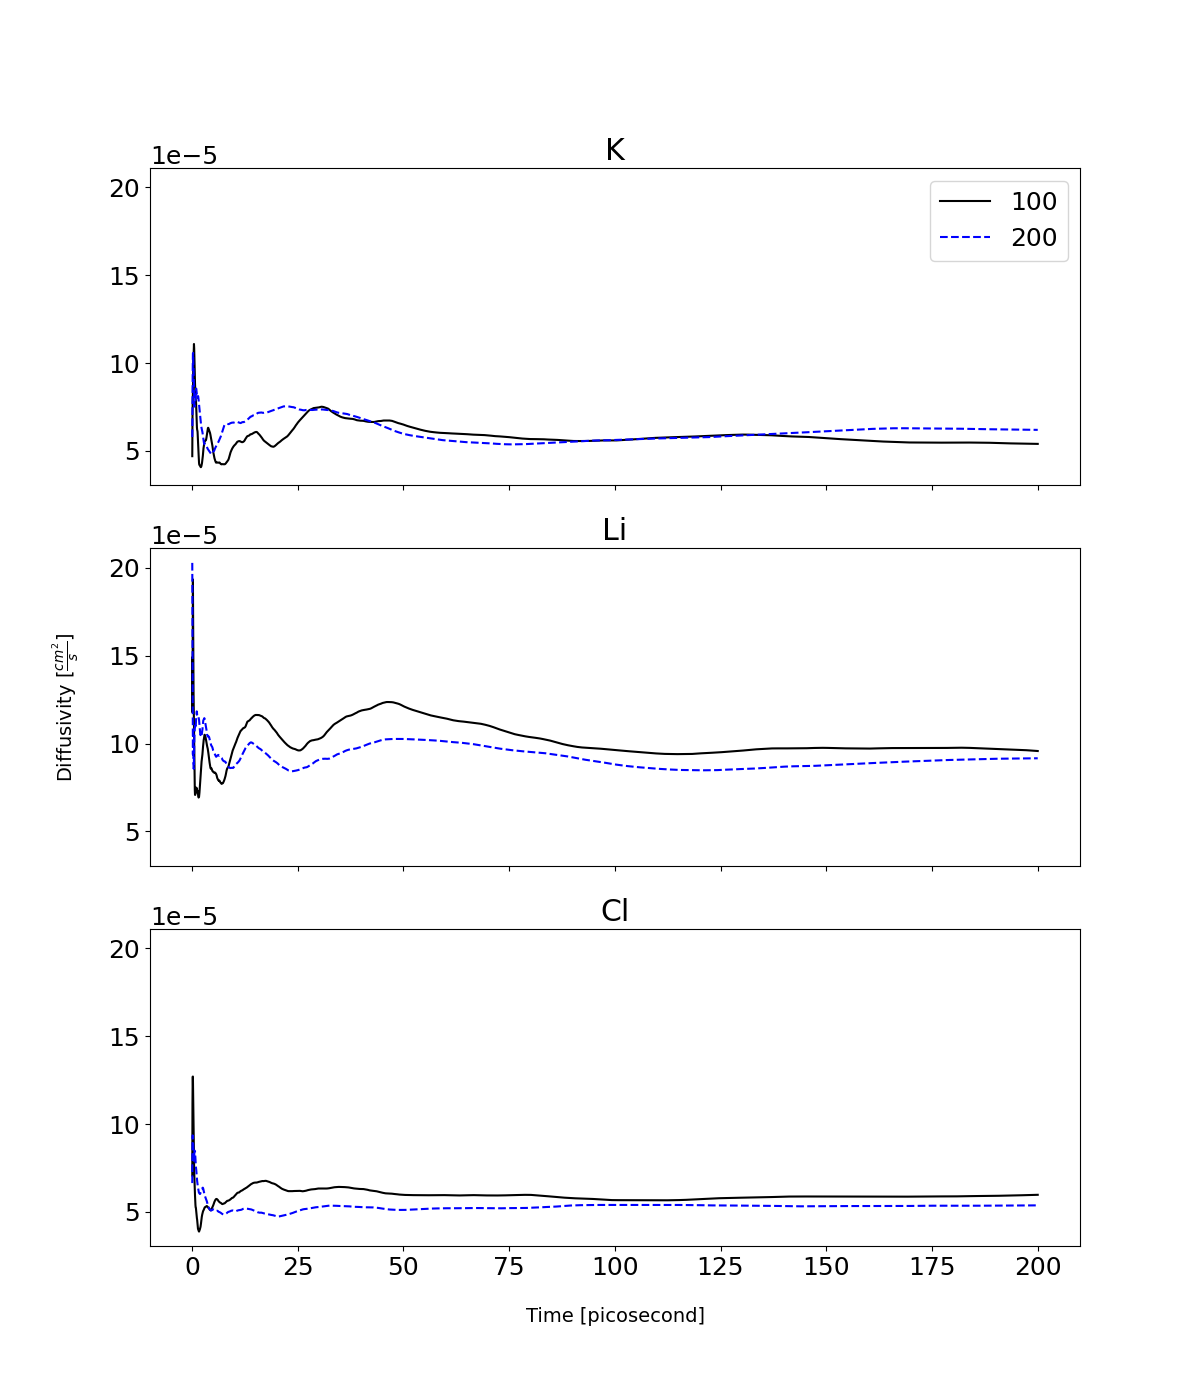
\includegraphics[width=0.8\textwidth]{100_vs_200_atoms.png} 
 \caption{The diffusion coefficient of each species of eutectic LiCl-KCl at 1200 K changing over time. The legend shows the number of atoms in the simulation cell.}
 \label{fig:100vs200}
\end{figure} 

Another aspect of the methodology to establish was the appropriate time increments of the simulation and if performing the simulations either in parallel or sequentially affected the result. A time increment in this nomenclature denotes the simulation time of a single simulation which will be combined with other simulations to construct a longer time trajectory. It has been shown that the accuracy of some physical quantities may be dependent upon the time increment \cite{Bengston2014}. In this study 25, 50, and 100 ps increments are considered due to the potential of time-dependent behavior. Bengston et al. \cite{Bengston2014} conducted a convergence study on simulation length in classical MD from 6 ps to 200 ps. The criteria they were studying were the error of temperatures, volumes, energies, pressures, and diffusion coefficient. For the diffusion coefficient, they determined that a 12 ps simulation length was sufficient while stating that it was only within the standard deviation of the 50 ps cases, but not the simulations of 100 or 200 ps. Due to this we have determined a need to ensure there is no time-dependent behavior that is being removed by only analyzing shorter simulations. From Fig. \ref{fig:100vs200}, it was determined that no time-dependent behavior lasted longer than 50 ps. This can be observed in Fig. \ref{fig:100vs200}, where there are extreme variations in the value of the diffusion coefficient for each ionic species over the first 25 ps and they last until 50 ps for the Li diffusion coefficient. However, it appears that a 25 ps trajectory may be missing key time-dependent behaviors. From this, it has been determined that 25 ps is not a long enough time increment and that a minimum of 50 ps increments should be used.

\begin{figure}[h!]
 \centering
 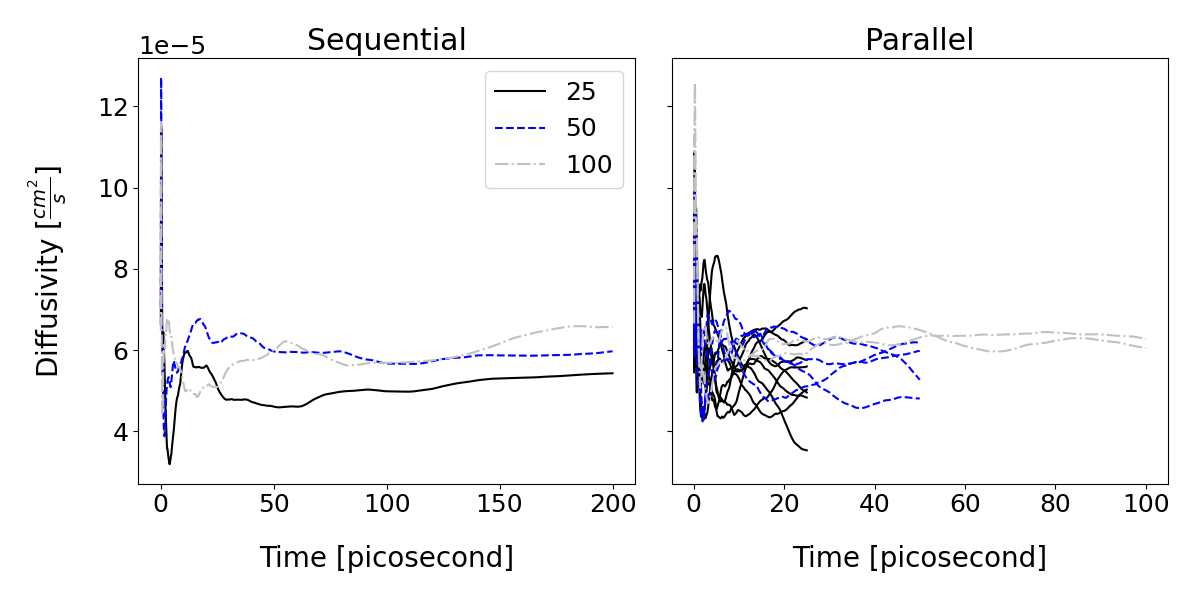
\includegraphics[width=0.8\textwidth]{SeqVsPar_Cl.png} 
 \caption{The total diffusion coefficient of eutectic LiCl-KCl at 1200 K for Cl ions changing over time. The legend shows the simulation increments in units of picoseconds.}
 \label{fig:SeqVsPar}
\end{figure} 

Fig. \ref{fig:SeqVsPar} shows the influence of sequential simulations (where one simulation is run and the end point of that simulation is utilized as the starting point of the next simulation) compared to parallel simulations where simulations are started from the same positions file and are allowed to evolve differently with unique initial velocity distributions. Both of these methods were utilized to simulate a total time of 200 ps, however, any potential time-dependent behaviors that are larger than the time increment in the parallel case would only be captured in the sequential simulations. When comparing the average diffusion coefficient value from the parallel simulations at 25, 50, or 100 ps they are within 1 standard deviation of the sequential simulations, with the exception of Li ions with a 50 ps increment, which can be seen in Table \ref{Table:parVSseq}. It must be noted that the standard deviation for the 100 ps increment is calculated from 2 values only. The sequential and parallel diffusion coefficient for the 50 ps increment for the Li ion (not shown) is within two standard deviations. This shows that the simulation method does not statistically influence the diffusion coefficient. Despite the fact that the 25 ps time increments showed reasonable agreement in \cref{fig:SeqVsPar}, the significant fluctuations below 25 ps in the sequential simulations indicate that time-dependent behavior may exceed 25 ps. The msd for the case with 100 atoms simulated in parallel where the four runs are averaged is shown in Fig. \ref{fig:averaged_msd}. This figure shows that all ion species have a linear msd, indicating a converged behavior with respect to time and the validity of using the Einstein equation. Thus, for the rest of this study, all simulations were run in parallel with a simulation length of 50 ps, and a total trajectory length of 300 ps.

\begin{figure}[h!]
 \centering
 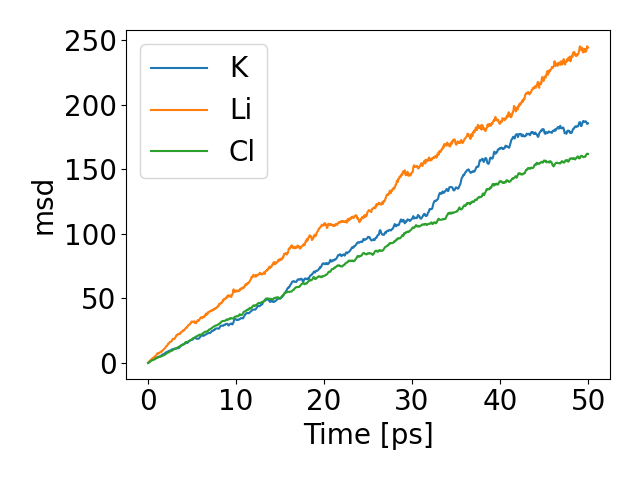
\includegraphics[width=0.7\textwidth]{msd_100_atoms_50ps_average.png} 
 \caption{The averaged mean squared displacement over the four unique runs for eutectic LiCl-KCl at 1200K with 100 atoms.}
 \label{fig:averaged_msd}
\end{figure} 

\FloatBarrier
\subsection{LiCl-KCl}
\subsubsection{Diffusion Coefficient}
The eutectic LiCl-KCl (43\%KCl) system was studied from 700-1300 K, with the diffusion coefficient plotted in Fig. \ref{fig:LiCl-KCl-diffusion}. In a diffusive regime, the log of the diffusion coefficient plotted against the inverse of temperature should be linear, and this behavior is seen in Fig. \ref{fig:LiCl-KCl-diffusion}. We can see that all ion types have an Arrhenius fit, which also serves to confirm that the system is in a diffusive regime. It can also be observed that Li has the largest diffusion coefficient and Cl has the smallest diffusion coefficient. Since there is no experimental data for the diffusion coefficient of eutectic LiCl-KCl at these temperatures in the literature, it is compared to other computational studies. Shown in Fig. \ref{fig:LiCl-KCl-diffusion} is the data collected by Bengston et al. \cite{Bengston2014}. As stated, the work by Bengston et al. is an AIMD study, but utilized significantly shorter time increments and smaller simulation cells than this work. Fig. \ref{fig:LiCl-KCl-diffusion} shows values of the diffusivity lower than those of Bengston but the same trends are present, in that Cl ion diffusion is the slowest and that Li ion diffusion is the fastest. The error bars on Fig. \ref{fig:LiCl-KCl-diffusion} for our data are the standard deviation of the diffusion coefficient from the six parallel simulations.
The beta parameter is shown in Table \ref{table:licl-kcl-beta}, and most of the beta parameter values are close to 1. The data at 700 K is the only temperature that has all ion types with a beta value below 0.9, which is likely due to the slower diffusion occurring at lower temperatures, and thus the data at 700 K should be used with caution. However, even the data at 700 K appears to follow the general Arrhenius trend of the truly diffusive high-temperature data, providing confidence in the presented results.

\begin{figure}[h!]
 \centering
 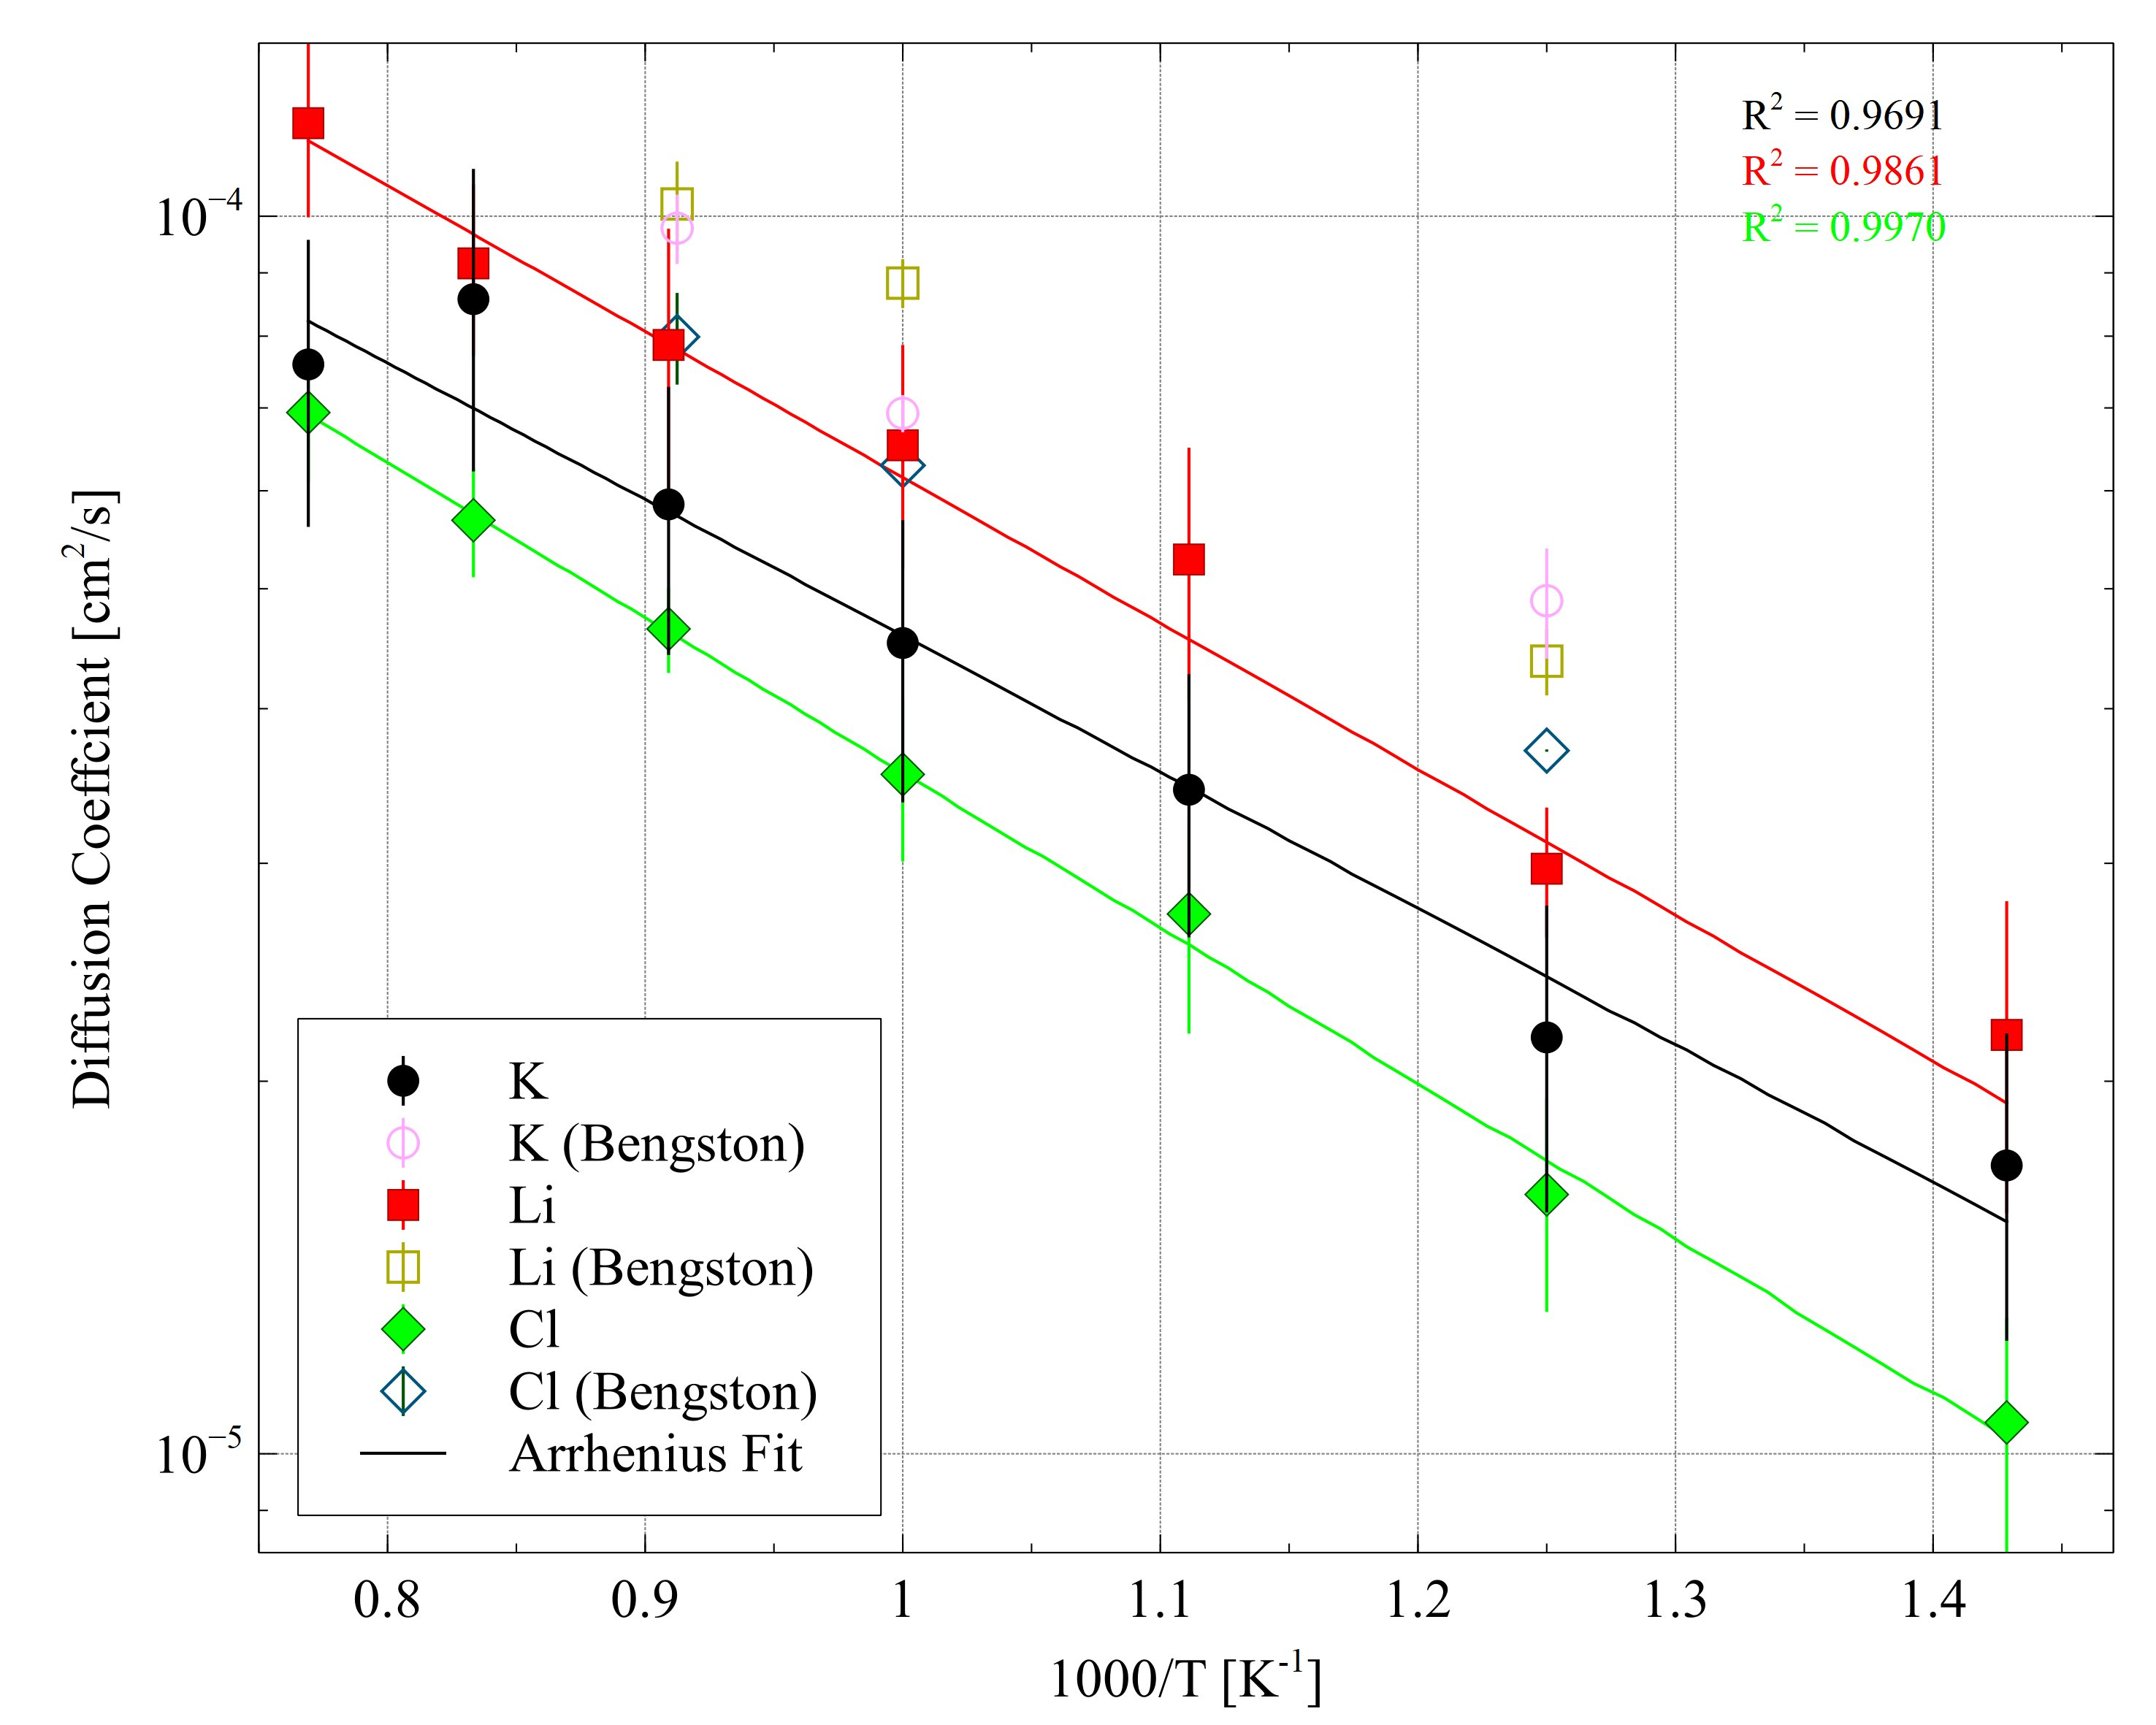
\includegraphics[width=0.8\textwidth]{diff_eutectic_licl_kcl.jpg} 
 \caption{The log of the diffusion coefficients of K, Li, and Cl ions in LiCl-KCl eutectic (closed markers) and their Arrhenius fits compared to the AIMD study by Bengston et al. \cite{Bengston2014} (open markers).}
 \label{fig:LiCl-KCl-diffusion}
\end{figure} 

The diffusion coefficients of K and Cl ions in KCl are shown in Fig. \ref{fig:KCl-diffusion}, which show that both K and Cl ions have Arrhenius behavior. It can not be determined in AIMD if the diffusion of K or Cl ions is faster as they fall within each other's standard deviation at each temperature and alternate which is larger at different temperatures. This behavior is also seen in the AIMD study of Bengston et al. \cite{Bengston2014}. The values of Bengston et al. are larger than the diffusion coefficients for both K and Cl ions that we report. When compared against experiment values reported by Janz \cite{janz_Diffusion} our AIMD study underestimates the diffusion coefficient for both K and Cl ions. It is unknown what the exact sources of discrepancy with experiment are. We strongly believe that the methods utilized here are more robust and thorough than those of Bengston, and thus should provide more accurate results. Thus, we would argue that Bengston’s methods overpredicted what the actual DFT-predicted diffusion coefficients are, which led to their results being “more accurate” compared to experiment. When comparing the K ions in the eutectic to KCl, it can be observed that K ions diffuse faster in the eutectic system. The diffusion of Cl ions in the eutectic and KCl systems falls within each other's standard deviation. The tabulated values for the diffusion coefficients of eutectic LiCl-KCl (Table \ref{Table: licl-kcl-eut diffusion}) and KCl (Table \ref{Table: kcl diffusion}) and beta parameters of the eutectic (Table \ref{table:licl-kcl-beta}) and KCl (Table \ref{table:licl and kcl-beta}) can be seen in the Appendix. It should be noted that only three data points were examined for the KCl system due to the higher melting point of KCl, which limited the minimum temperature to 1100 K. 

\begin{figure}[h!]
 \centering
 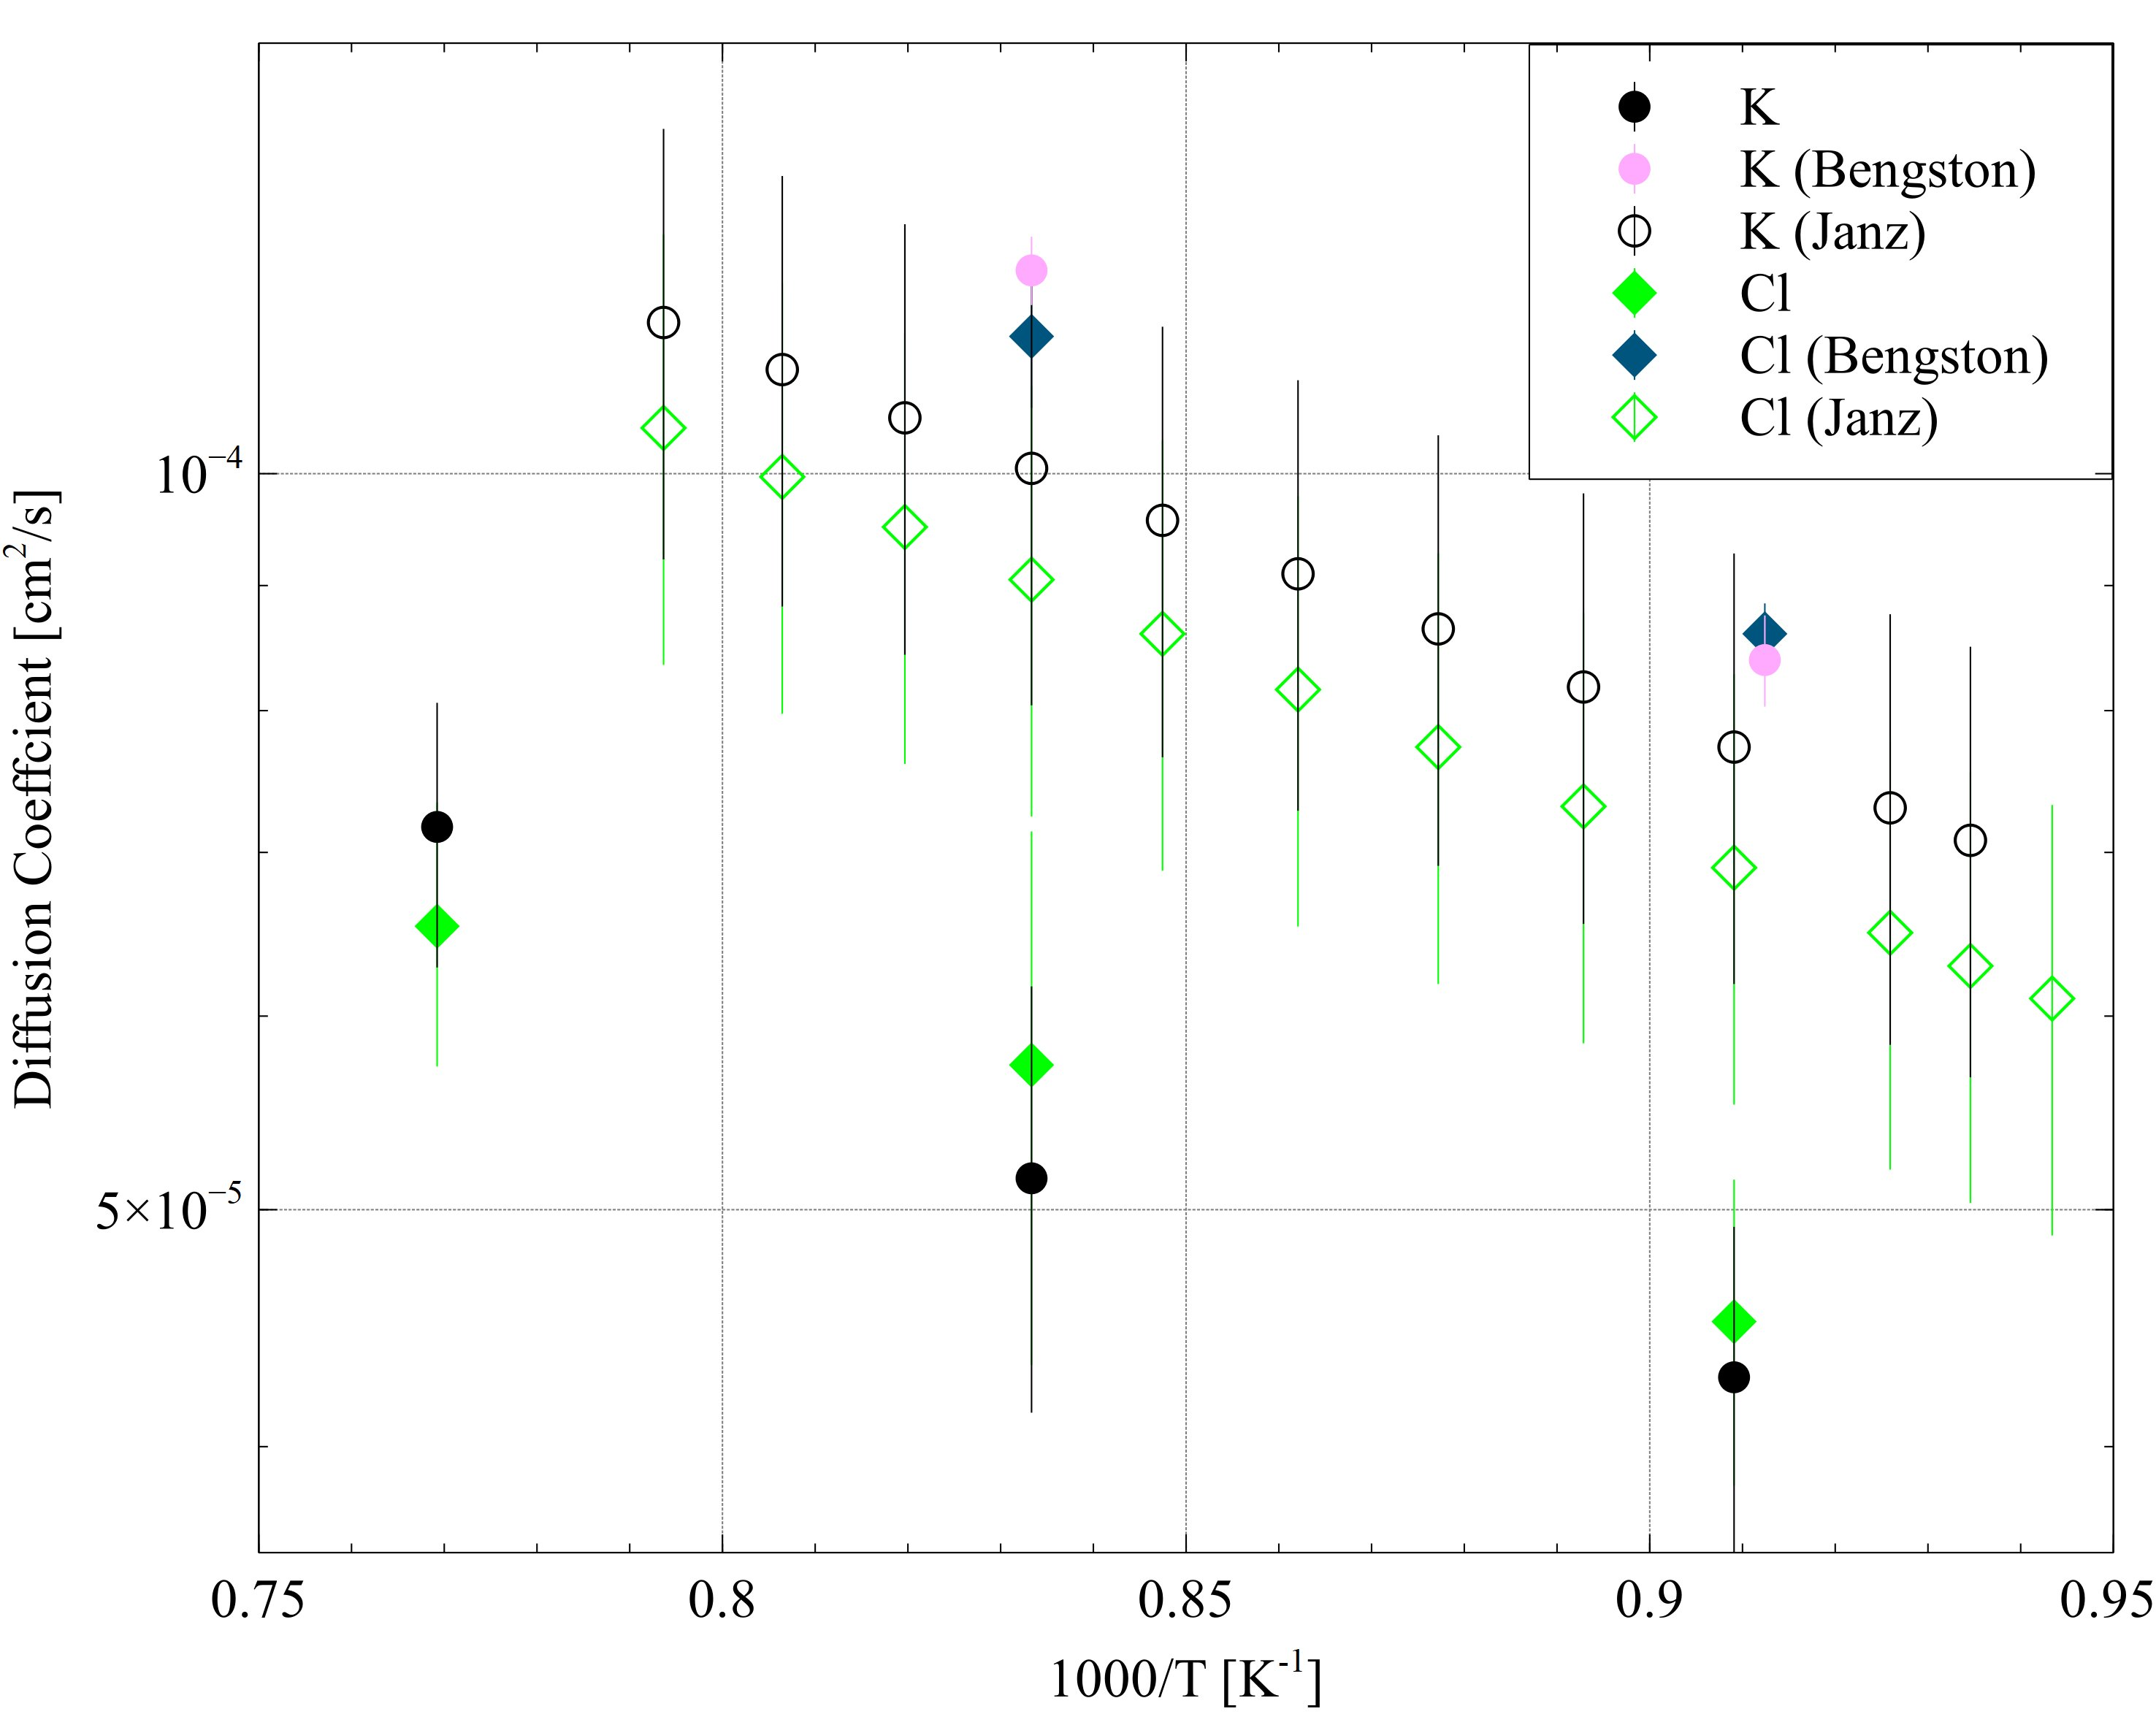
\includegraphics[width=0.7\textwidth]{diff_kcl.jpg} 
 \caption{The diffusion coefficients of K, and Cl ions in KCl compared against experimental results from Janz \cite{janz_Diffusion} and AIMD results from Bengston et al. \cite{Bengston2014}. Closed markers are AIMD and open markers are experimental results.}
 \label{fig:KCl-diffusion}
\end{figure}

The diffusion coefficient of LiCl can be seen in Fig. \ref{fig:LiCl-diffusion}. It can be observed that both Li and Cl ions have an Arrhenius behavior. It can also be noted that Li diffuses faster than Cl ions. The AIMD values for Li ions slightly underestimate the extrapolated data from Janz \cite{janz_Diffusion} but would fall within the reported 20\% uncertainty of the experimental data. The Li ions overlap with Bengston et al. \cite{Bengston2014} at 1100 K. The Cl ions are also underestimating the extrapolated data from Janz and Bengston. There is a significant difference in the slope of the diffusion coefficient of Cl ions when compared to Janz \cite{janz_Diffusion}. The slope is defined as the activation energy in \cref{eq:Ea}, and our work estimates a value of 0.189 $\pm$ 0.39 for Cl in LiCl, while Janz reports a value of 0.139 $\pm$ 0.36. Contrary to the K ions which diffuse faster in the eutectic than KCl, the Li ions diffuse faster in the LiCl system than the eutectic. The Cl ion diffusion coefficient for both the LiCl and eutectic system fall within each other's standard deviation.

\begin{figure}[h!]
 \centering
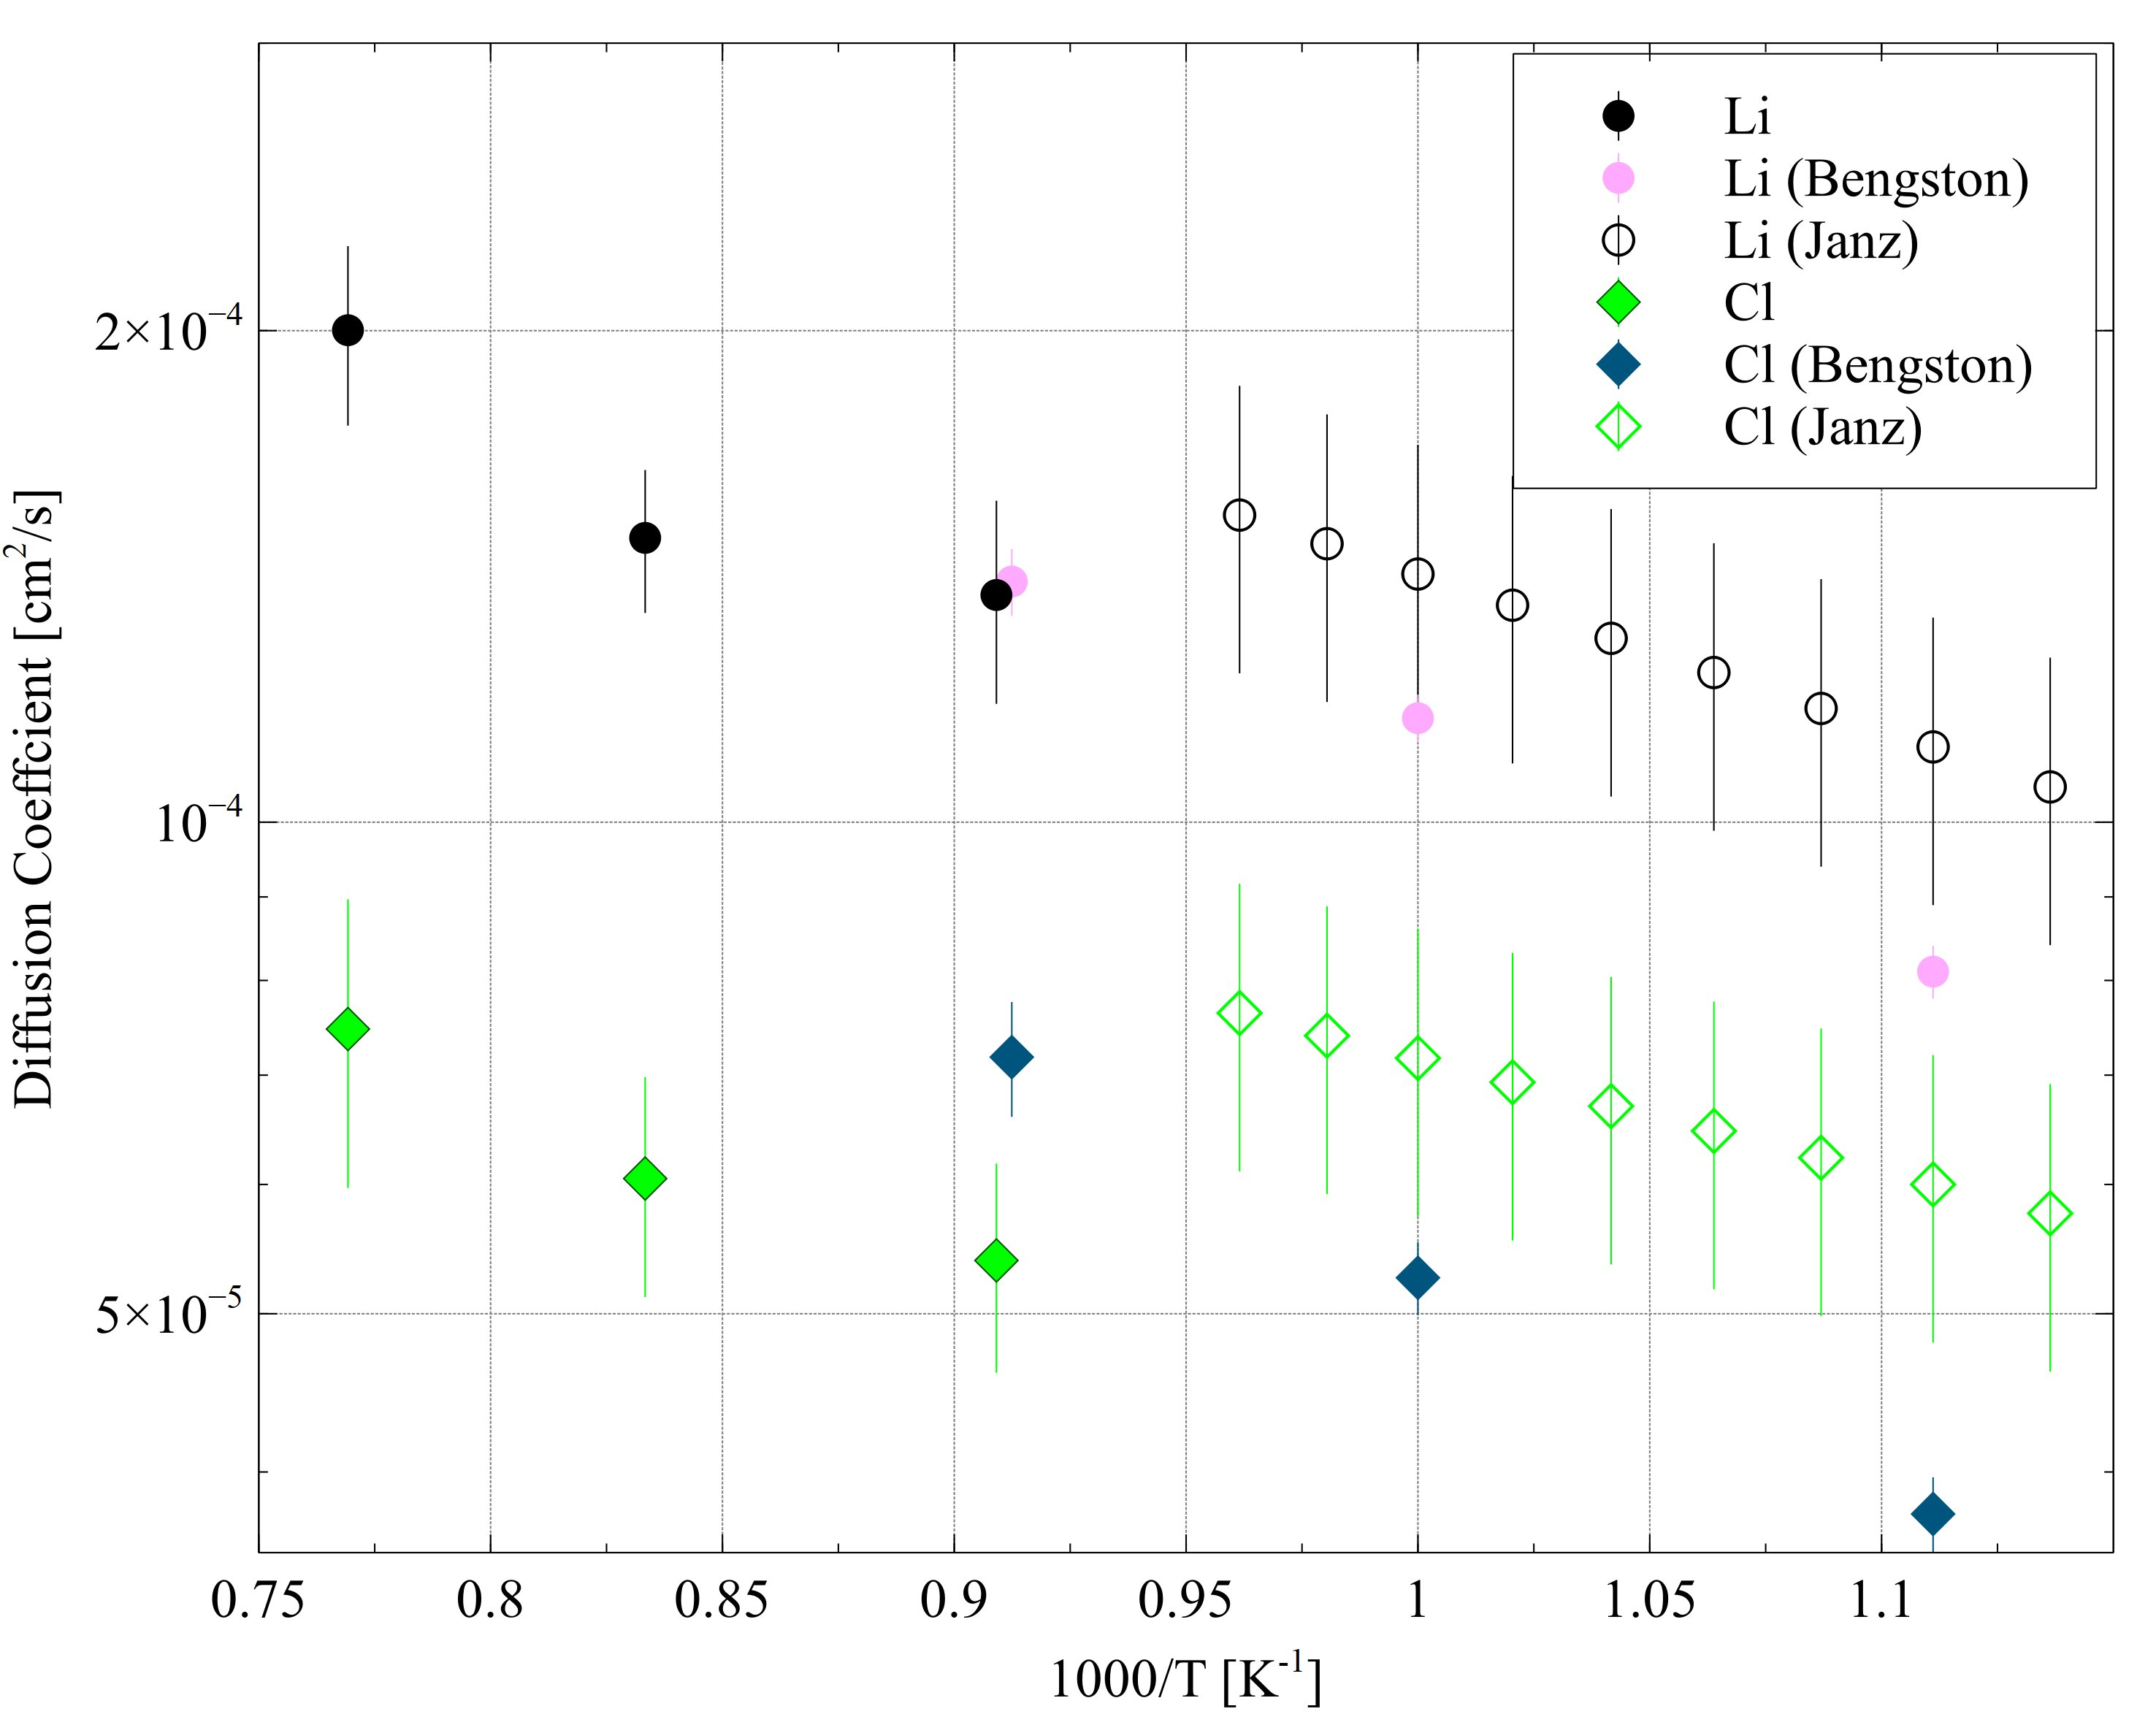
\includegraphics[width=0.7\textwidth]{diff_licl.jpg} 
 \caption{The diffusion coefficients of Li, and Cl ions in LiCl compared against experimental results from Janz \cite{janz_Diffusion} and AIMD results from Bengston et al. \cite{Bengston2014}. Closed markers are AIMD and open markers are experimental results.}
 \label{fig:LiCl-diffusion}
\end{figure}


The total diffusion coefficients for LiCl, KCl, and eutectic can be seen in Fig. \ref{fig:likcl_total_diff}. What can be observed here is that the LiCl system displays faster diffusion than the eutectic and KCl is the slowest of the three. The eutectic total diffusion coefficient is compared to the total diffusion calculated through the linear interpolation between the endpoints for comparison purposes. It appears that the eutectic shows diffusivity that is slightly lower than linear interpolation would predict, which indicates the possibility of non-ideal mixing behavior with regard to diffusive properties. 

\begin{figure}[h!]
 \centering
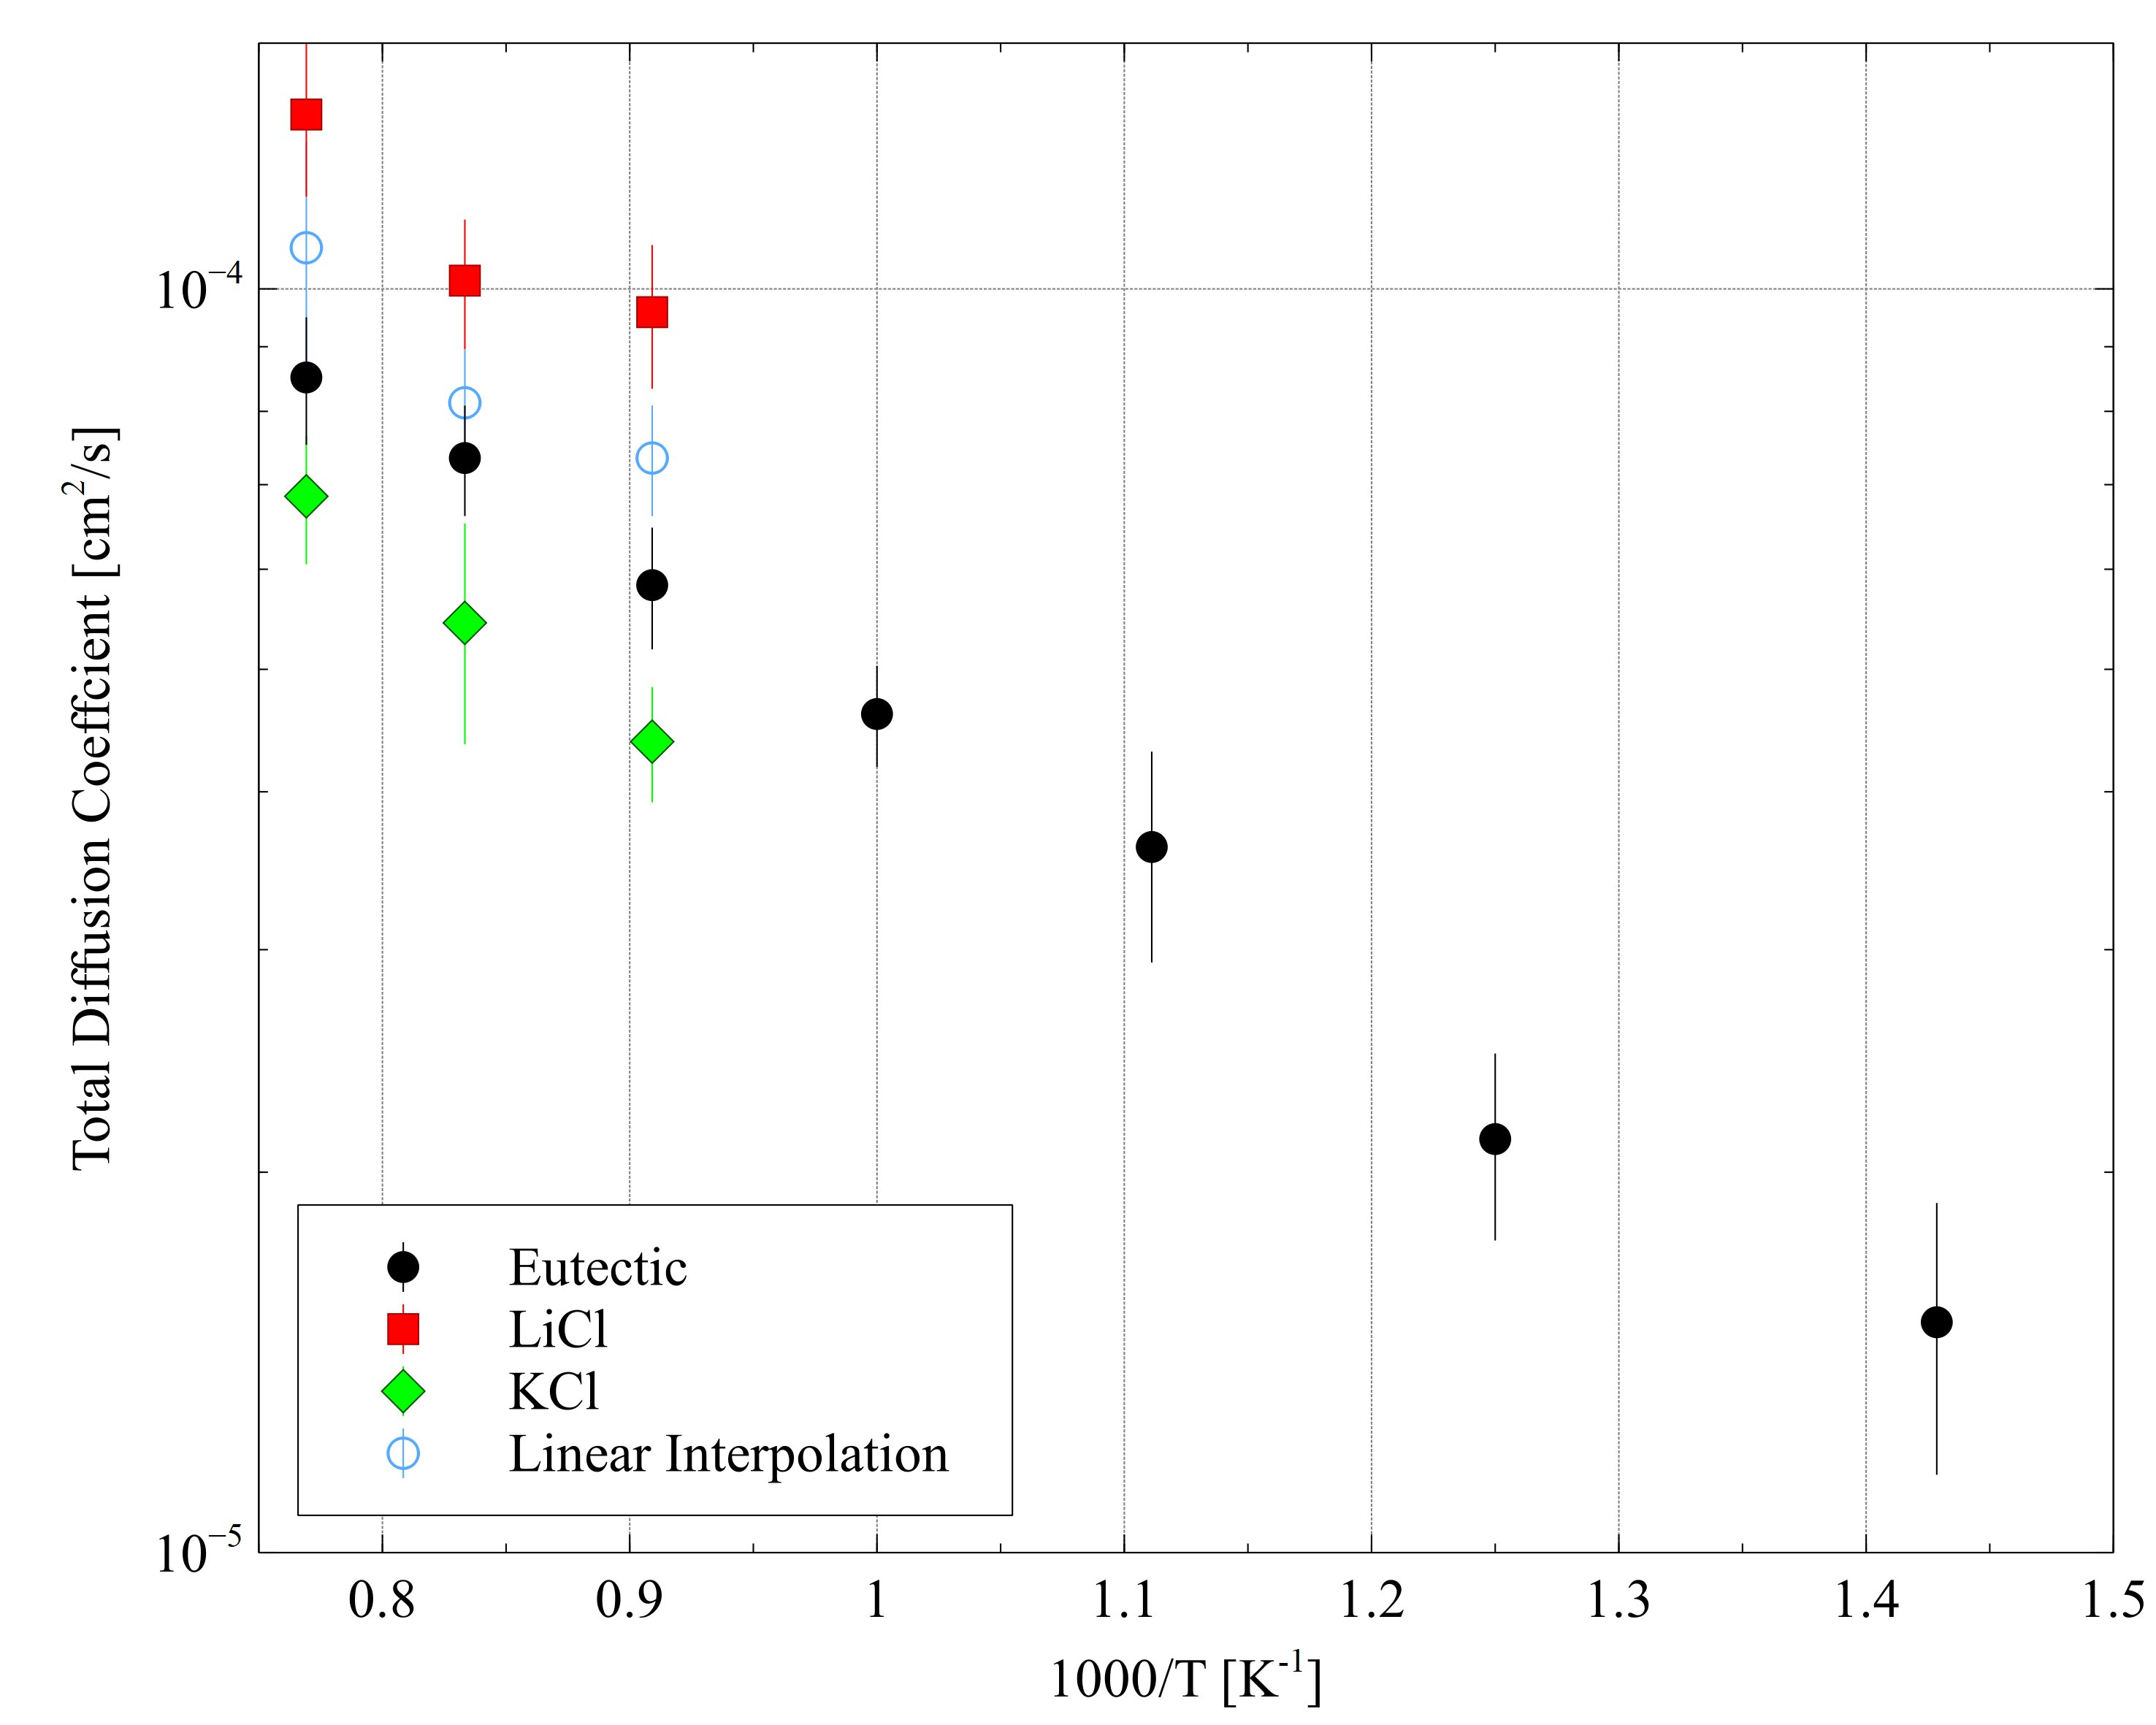
\includegraphics[width=0.7\textwidth]{diff_total_likcl.jpg} 
 \caption{The total diffusion coefficients of LiCl, KCl, eutectic LiCl-KCl. The eutectic value is compared to the value calculated via linear interpolation of the endpoints.}
 \label{fig:likcl_total_diff}
\end{figure}
\FloatBarrier

The activation energy and the pre-exponential factor for the diffusion coefficient in Eq. \ref{eq:Ea} are provided in Table \ref{table:activation_energy}. It must be noted that the LiCl and KCl systems have only three temperature points for the fit of an Arrhenius equation, which causes the calculated activation energy to be sensitive to the diffusion coefficient value at any given temperature. What we can see in this table is that in KCl the activation energy of the K ion is overestimated compared to the experimental value \cite{janz_Diffusion} by 8\%, while the activation energy for the Cl ion is underestimated by 26\%, and the pre-exponential factor is underestimated for both ions. For the LiCl system, the difference in the Li ion activation energy is 23.3\% and for Cl ions it is 36\%. For the pre-exponential factor, the difference is 18.9\% for Li and 8.3\% for Cl ions. The LiCl-KCl eutectic system is compared against the Bengston et al. \cite{Bengston2014} AIMD study as there are no experimental studies to compare against. The differences in the activation energy for Li, K, and Cl ions are 8.3\%, 32.9\%, and 25.8\% respectively. The data from Bengston only had three data points which could explain some of the large differences between the two values. It should also be emphasized that there are only the single experimental values from Janz for comparison to this data set, which includes estimated errors of 20\%. 

\begin{table}[h!]
\centering
\caption{The activation energy (E$_a$) and pre-exponential factor (D$_0$) (\cref{eq:Ea}) for LiCl, KCl, LiCl-KCl eutectic, NaCl, MgCl$_2$, and NaCl-MgCl$_2$ eutectic, compared to computational \cite{Bengston2014} and experimental \cite{janz_Diffusion} results. }
\begin{tabular}{|c|c|c|c|c|}
\hline
System& Species & E$_a$ [eV] & D$_0$ [10$^3$ cm$^2$/s] &reference\\
\hline
LiCl & Li & 0.233 (0.245, 0.189) & 1.51 (1.92, 1.27) & This Work (\cite{Bengston2014},\cite{janz_Diffusion}) \\
     &   Cl  &0.189 (0.273, 0.139) & 0.39 (0.12, 0.36) & This Work (\cite{Bengston2014},\cite{janz_Diffusion}) \\
\hline

KCl & K              &   0.323 (0.299) &    1.26 (1.8)  &   This Work (\cite{janz_Diffusion}) \\
    &Cl             &   0.230 (0.309)  &    0.51 (1.8)  &   This Work (\cite{janz_Diffusion})\\

\hline
LiCl-KCl    &Li    &0.234 (0.214) &   0.93 (1.05)  &    This Work (\cite{Bengston2014})\\
            &K     &0.219 (0.147) &   0.58 (0.40)  &    This Work (\cite{Bengston2014})\\
            &Cl    &0.249 (0.185) &   0.64 (0.54)  &    This Work (\cite{Bengston2014})\\
\hline
NaCl    &Na    &   0.285 (0.310)  &   0.93 (2.1)   &  This Work (\cite{janz_Diffusion})\\
        &Cl    &   0.266 (0.322)  &   0.46 (1.9)   &   This Work (\cite{janz_Diffusion})\\
\hline
MgCl$_2$    &Mg   &   0.324   &   0.51   &   This Work\\
            &Cl    &   0.319   &   0.48    &   This Work\\
\hline
NaCl-MgCl$_2$   &Na    &   0.150   &   0.26    & This Work\\
                &Mg   &   0.247   &   0.28    &   This Work\\
                &Cl    &   0.244   &   0.32    &   This Work\\
\hline
\end{tabular}

\label{table:activation_energy}
\end{table}

\FloatBarrier
\subsubsection{Viscosity}
The viscosity for the LiCl-KCl system is shown in Fig. \ref{fig:LiCl-KCl visc} including the eutectic composition along with the two endpoint salts, LiCl and KCl. The solvodynamic radii (R) in \cref{eq:SES} can be approximated to half the first peak distance on the rdf, which is the mole fraction average for all the ionic species in the salt. The numerical values for the solvodynamic radii are reported in Table \ref{Table:solvodynamic}. It can be observed that the solvodynamic radii decrease as the temperature decreases. What can be observed is that the viscosity of KCl is the largest, LiCl has the smallest viscosity, and the eutectic falls in the middle. This trend is not observed in the experimental values \cite{janz_visc,janz_nist,janz_osti,kim2012high,brockner1975high,Tasidou}. What the experiments show is that KCl does have the largest viscosity but the viscosity for LiCl and the eutectic are approximately the same and at the higher temperatures, the eutectic has a smaller value (but is still within the error bars of the LiCl viscosity value). It can be observed that calculating the viscosity via the Stokes-Einstein-Sutherland relation (\cref{eq:SES}) potentially underestimates the viscosity reported in Janz \cite{janz_visc}. It should be noted that Janz reported data for 40\%mol KCl, while the values from Kim et al. \cite{kim2012high} are for the eutectic composition. It can be observed that the viscosity of LiCl is likewise underestimated when compared against experimental work from Tasidou \cite{tadano2014anharmonic} and Janz \cite{janz_nist,janz_osti}, as well as the fit from Brockner et al. \cite{brockner1975high}. However, we see good agreement with the experiment for the viscosity of KCl when comparing to both Janz \cite{janz_nist} and Tasidou et al. \cite{Tasidou}. Regardless, additional experimental data is warranted to verify the existing literature since only a single study has been performed for this system in the past forty years.Another point to consider is that the method used for the calculation of the viscosity has underlining assumptions and one of the reasons that the viscosity could differ more with LiCl is that this is a highly correlated solvent which means that some of the assumptions discussed in Section 1 won't be as applicable. This could be a cause for the discrepancy observed for LiCl.
\begin{figure}[h]
 \centering
 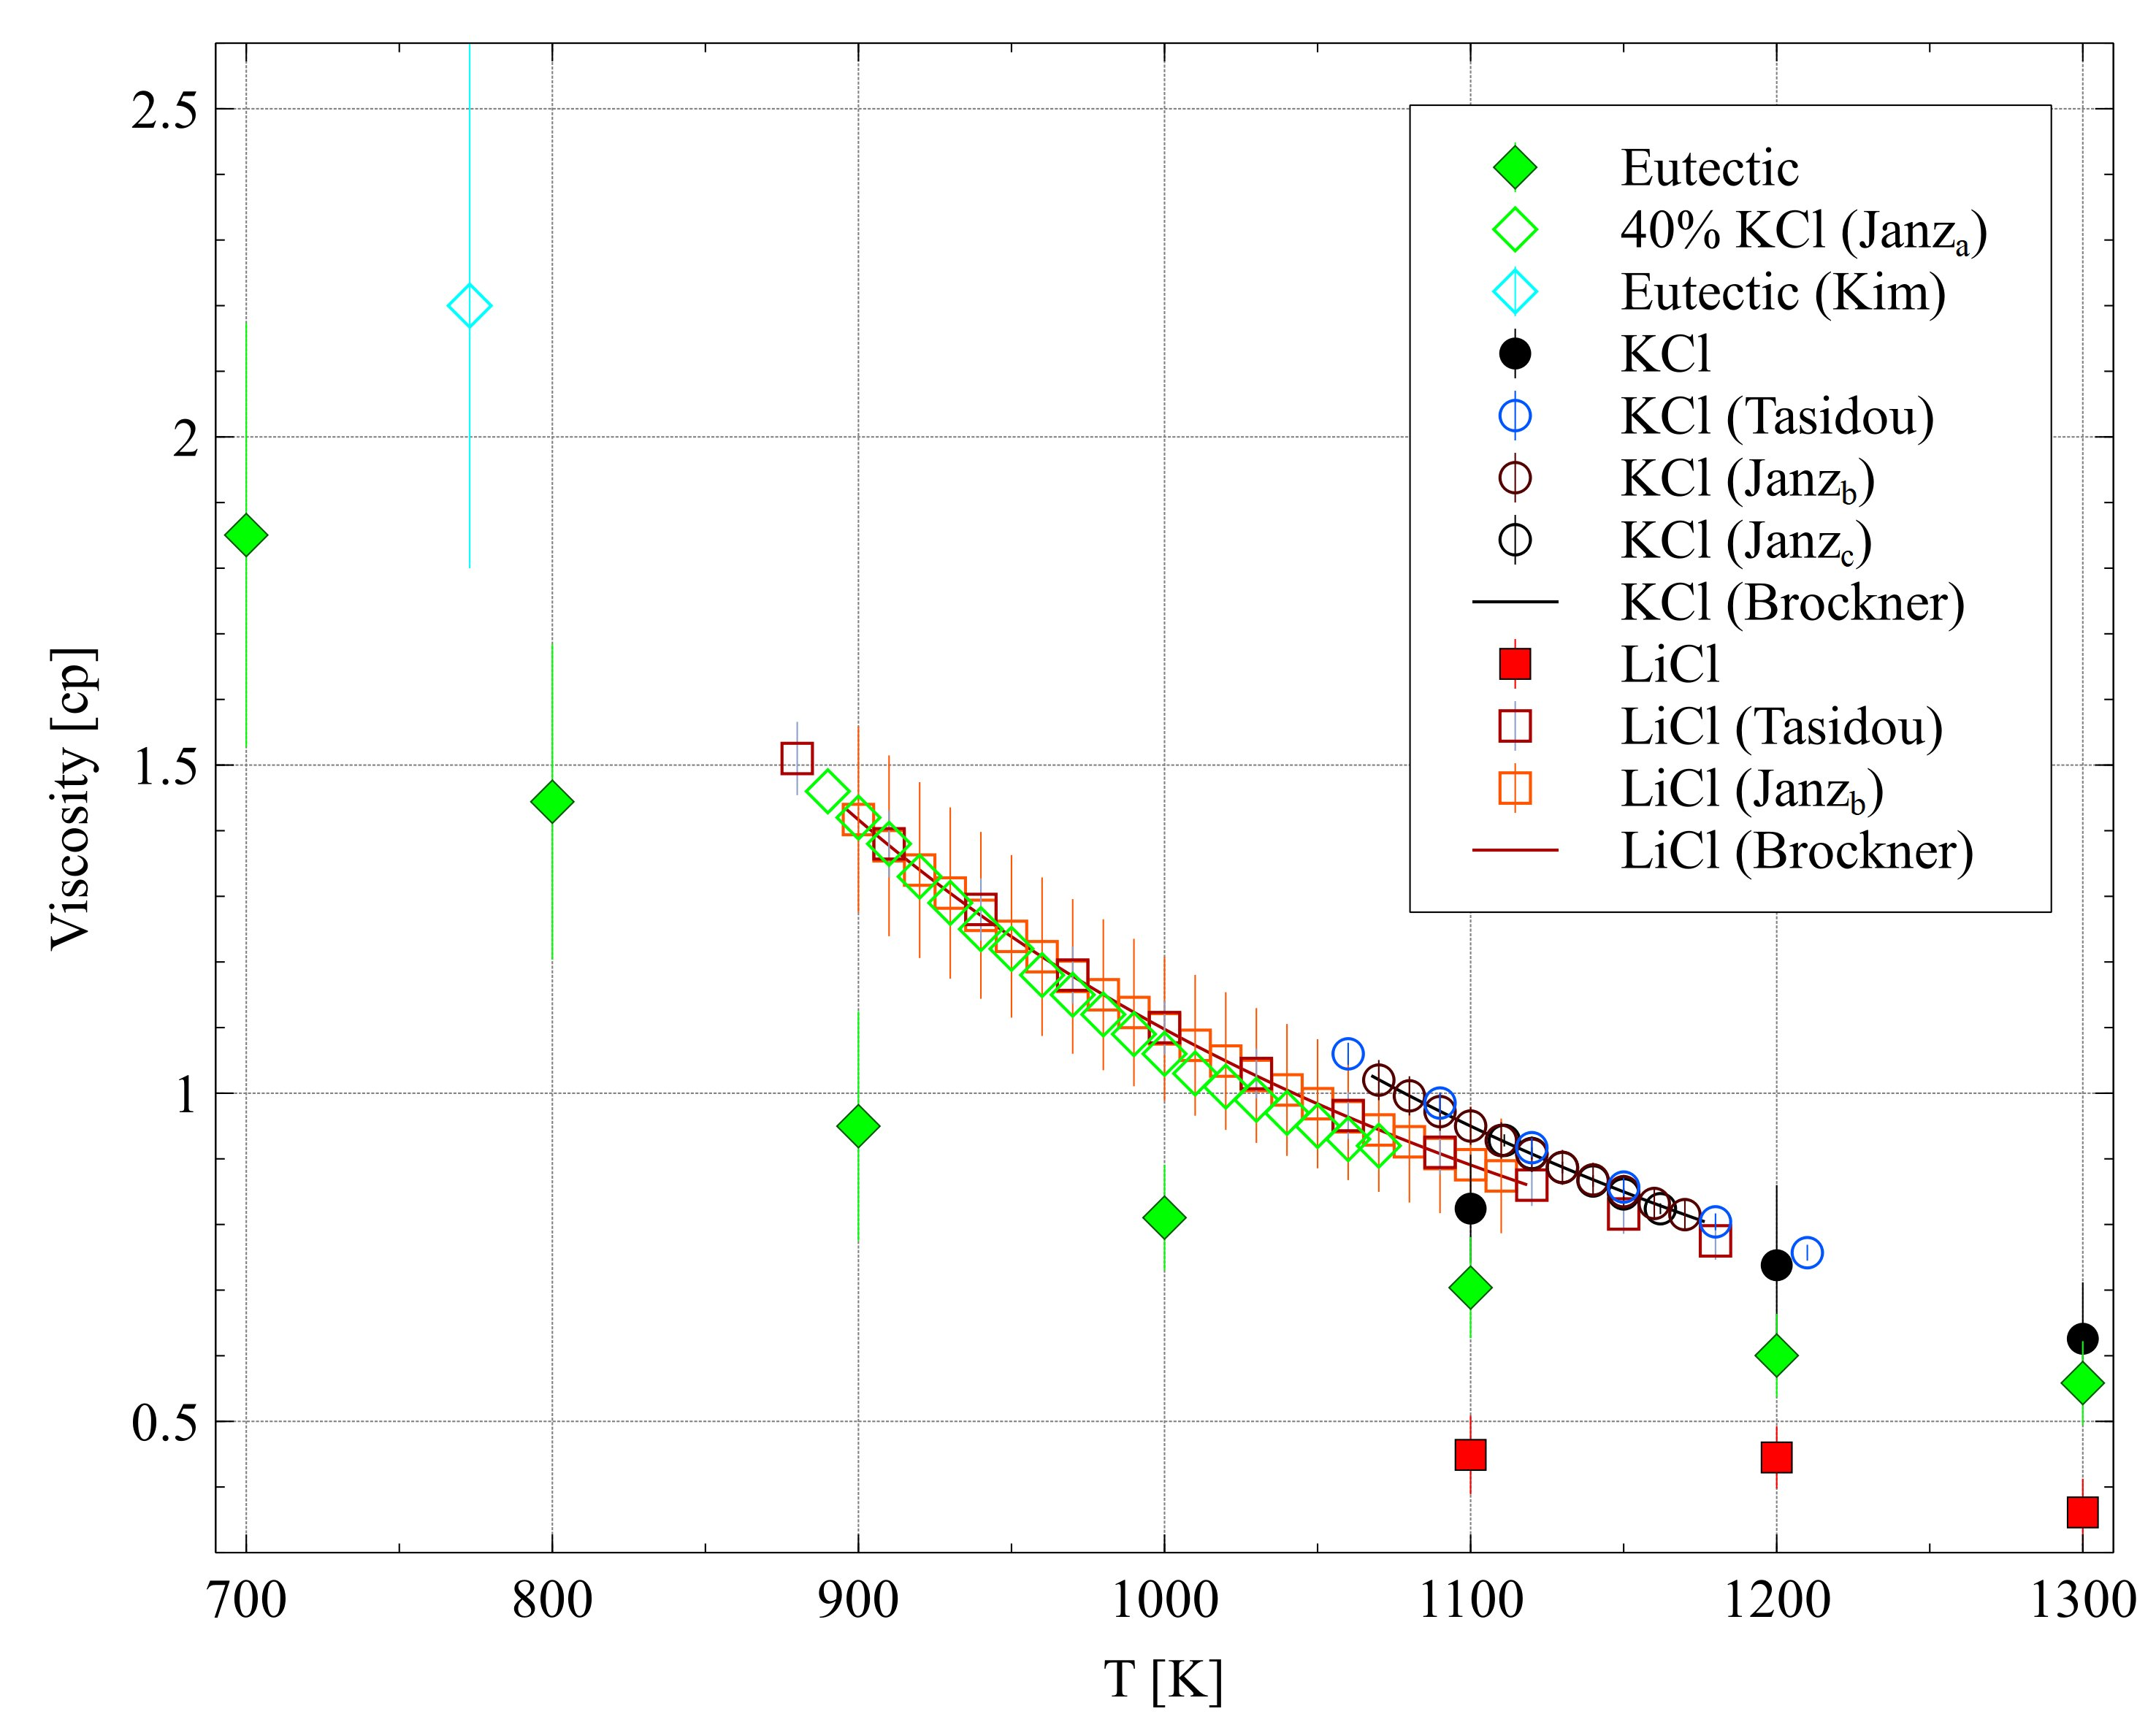
\includegraphics[width=0.7\textwidth]{visc_licl-kcl.jpg} 
 \caption{The viscosity for LiCl-KCl eutectic, KCl, and LiCl. The solid marks are from this work, the hollow markers are experimental data, and the solid lines are experimental fits from Janz at 40\%mol KCl \cite{janz_visc}, the eutectic composition from Kim et al. \cite{kim2012high}, and for LiCl and KCl from Tasidou et al. \cite{Tasidou}, Janz \cite{janz_nist,janz_osti} and Brockner et al. \cite{brockner1975high}.}
 \label{fig:LiCl-KCl visc}
\end{figure} 

\FloatBarrier
\subsubsection{Heat Capacity}
Both the isochoric ($C_V$) and the isobaric ($C_P$) heat capacities can be seen in Fig. \ref{fig:LiCl-KCl cv}. For the isobaric heat capacity the values of \textit{$\alpha$} and \textit{$\beta_T$} were used from our prior work on LiCl-KCl \cite{duemmler_liclkcl} while the ($C_V$) values were calculated using \cref{eq:cv}. For $C_V$ for 1100 - 1300 K, the values are very similar for the eutectic, LiCl, and KCl systems. It can also be observed that the $C_V$ values are lower than the calculated $C_P$ values and the $C_P$ values found in the literature \cite{clark1973heats,janz_osti}, as expected. For the LiCl and KCl systems, there is no statistically significant dependence on temperature for the heat capacity as the standard deviation of the heat capacities at 1300 K overlaps with the data point at 1100 K. Likewise, the heat capacity for the eutectic composition has no statistically significant temperature dependence, but does show a statistically insignificant negative trend with temperature. The behavior reported for the eutectic $C_P$ value in our previous work \cite{duemmler_liclkcl} (utilizing a different methodology) shows a negative temperature dependence. The calculated isobaric heat capacity compares well with the experimental data from Janz et al. \cite{janz_osti} for LiCl and KCl and with Clark \cite{clark1973heats}, for the eutectic composition. In all cases where there is overlapping temperature data, the calculated $C_P$ values fall within the error bars of the experimental studies. Like the isochoric heat capacities, the isobaric heat capacity does not show statistically significant temperature dependence.


\begin{figure}[h]
 \centering
 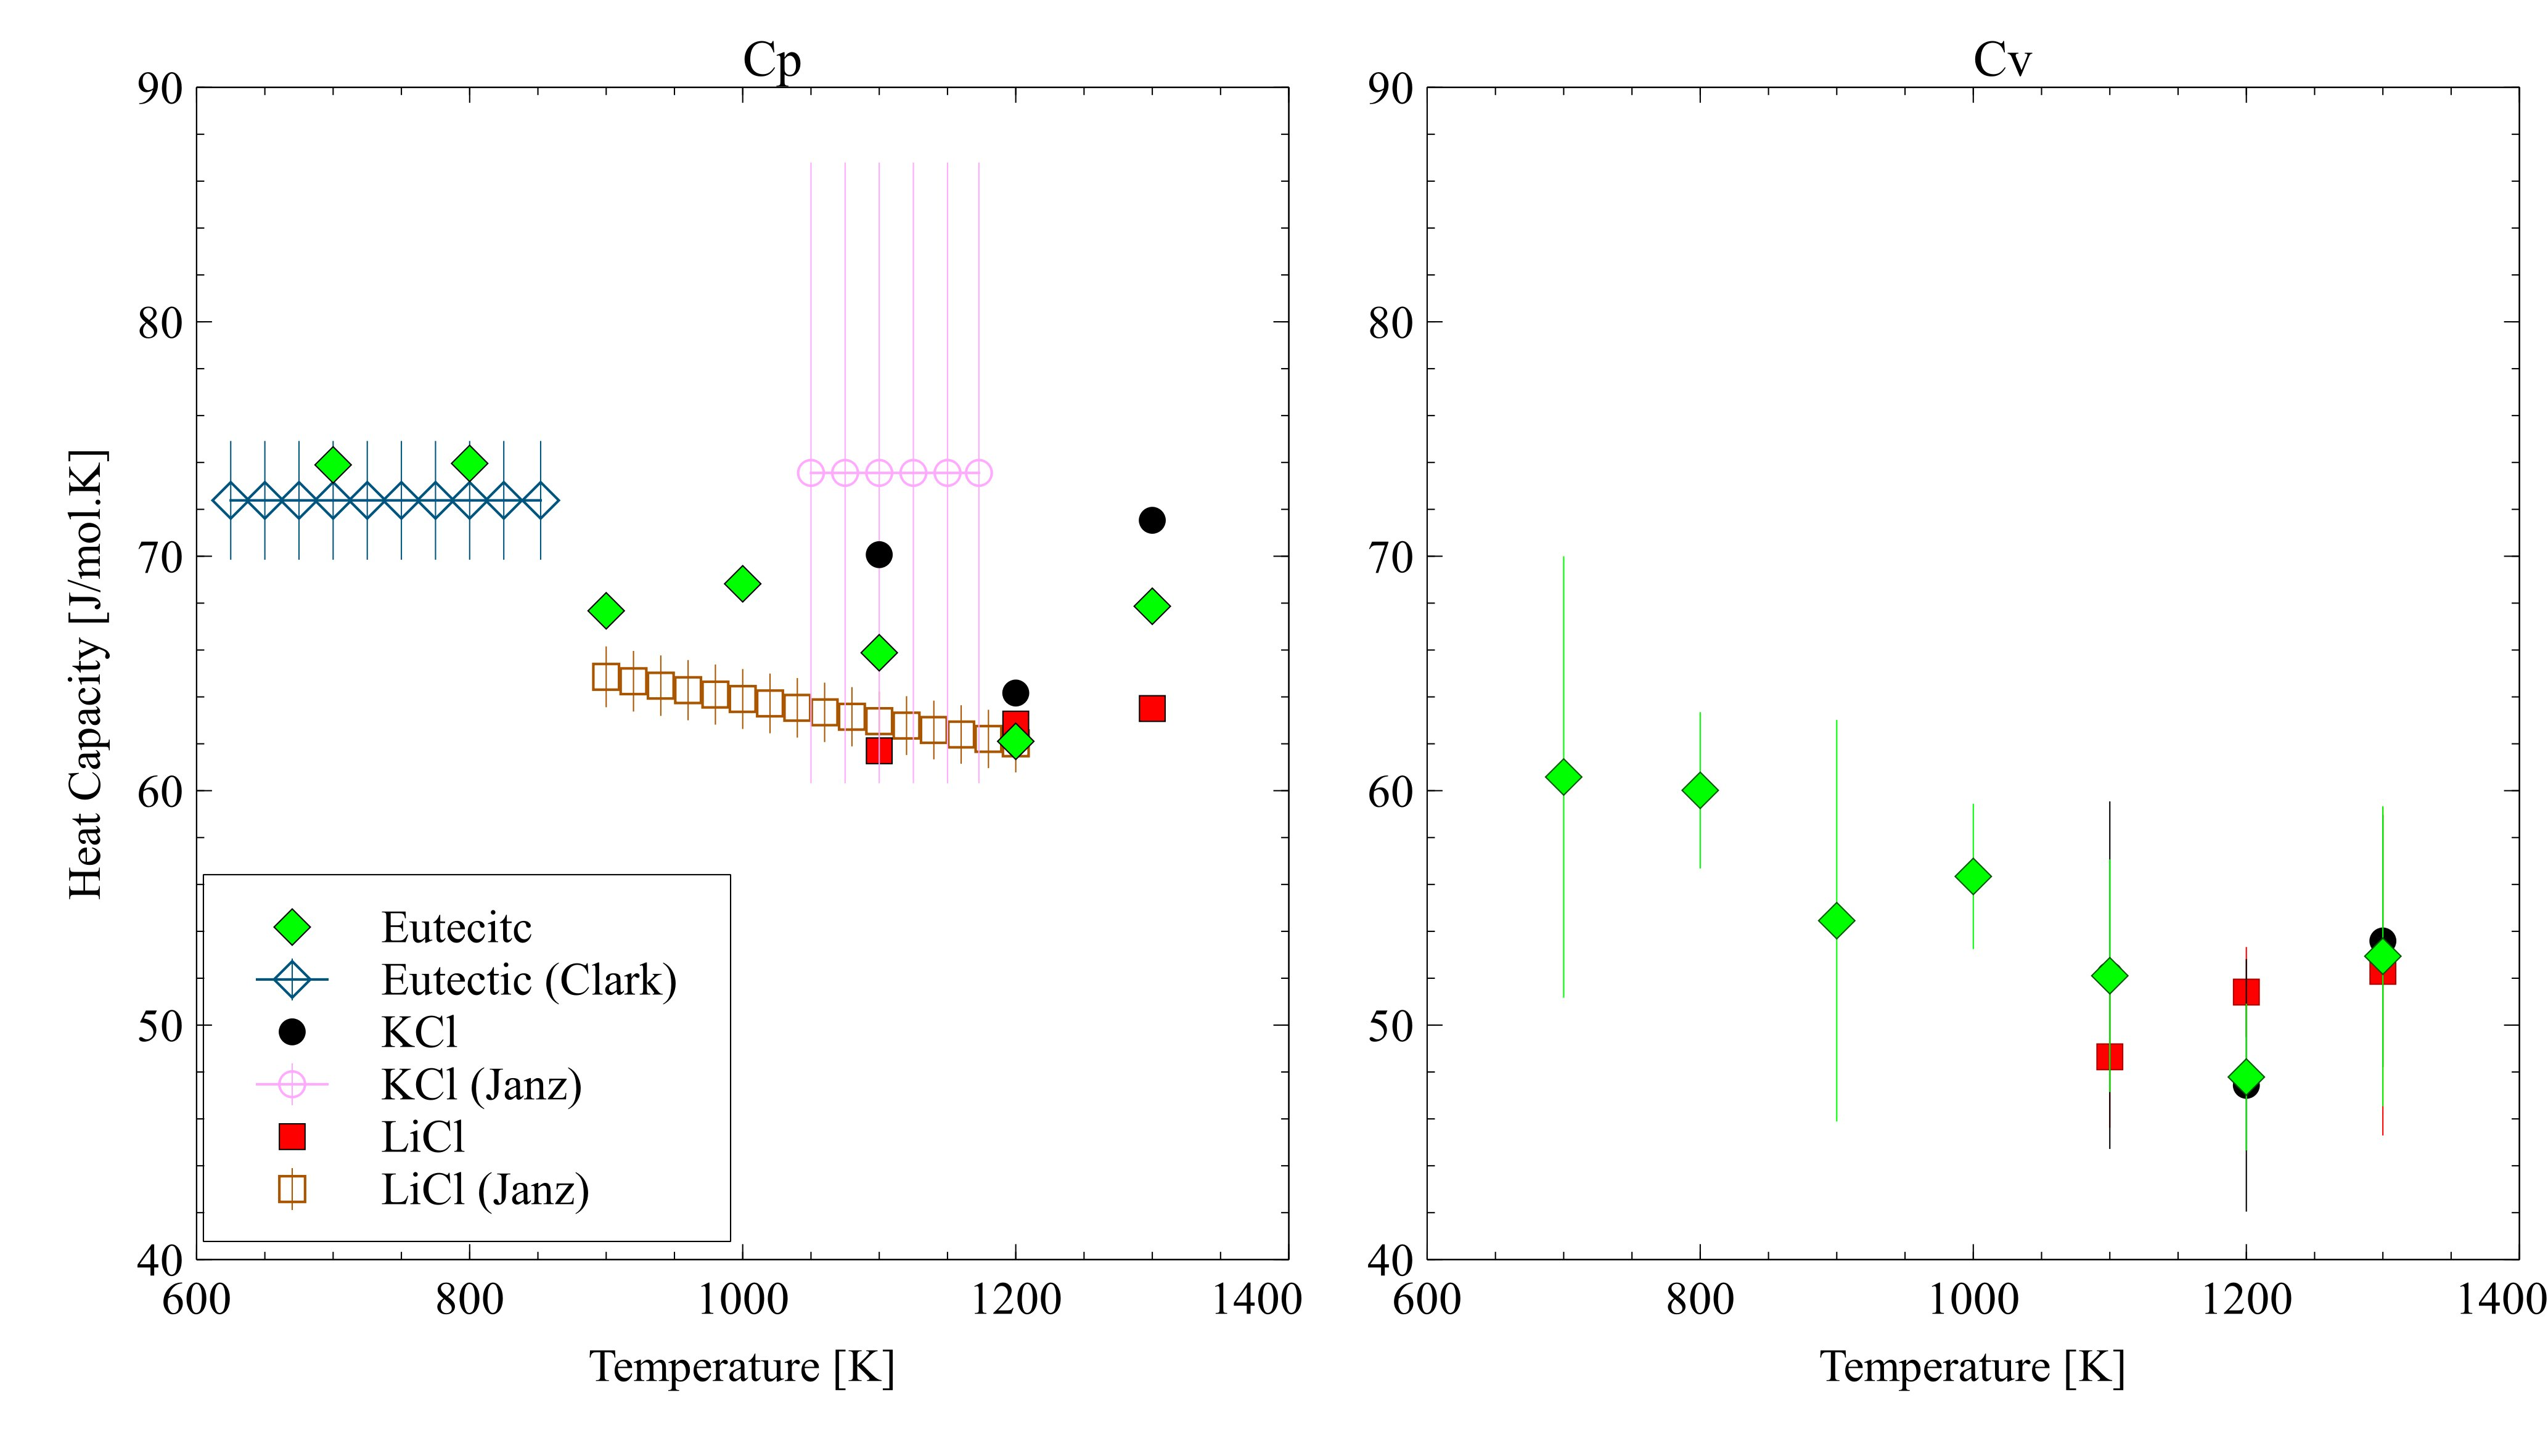
\includegraphics[width=0.9\textwidth]{cv_licl-kcl.jpg} 
 \caption{The isobaric (C$_P$) and isochoric (C$_V$) heat capacities for LiCl-KCl eutectic, LiCl, and KCl systems. The isobaric heat capacity is compared against experimental $C_P$ values \cite{janz_osti,clark1973heats}. Closed markers are AIMD results and open are experimental values.}

 \label{fig:LiCl-KCl cv}
\end{figure} 

\FloatBarrier
\subsection{NaCl-MgCl$_2$}
\subsubsection{Diffusion Coefficient}
The NaCl-MgCl$_2$ systems were studied from 1100-1300 K. The diffusion coefficients for NaCl-MgCl$_2$ eutectic (42.7\% MgCl$_{2}$), NaCl, and MgCl$_2$ can be seen in Fig. \ref{fig:NaCl-MgCl2-diffuion}. For the eutectic composition, we see that the diffusion coefficient ion order is Na $>$ Cl $>$ Mg. This is in agreement with the AIMD study from Xu et al. \cite{xu2020powerful} at lower temperatures. If their data is extrapolated with an Arrhenius fit, as shown in Fig \ref{fig:NaCl-MgCl2-diffuion}, their data slightly overestimates the diffusion coefficient compared to this work. Given the uncertainties in the data from this work and from Xu, this is considered a reasonable agreement. The beta parameter can be seen in Table \ref{table:nacl-mgcl2-beta} for reference. There are no experimental diffusion coefficient studies for the NaCl-MgCl$_2$ system available for comparison.
\begin{figure}[!h]
 \centering
 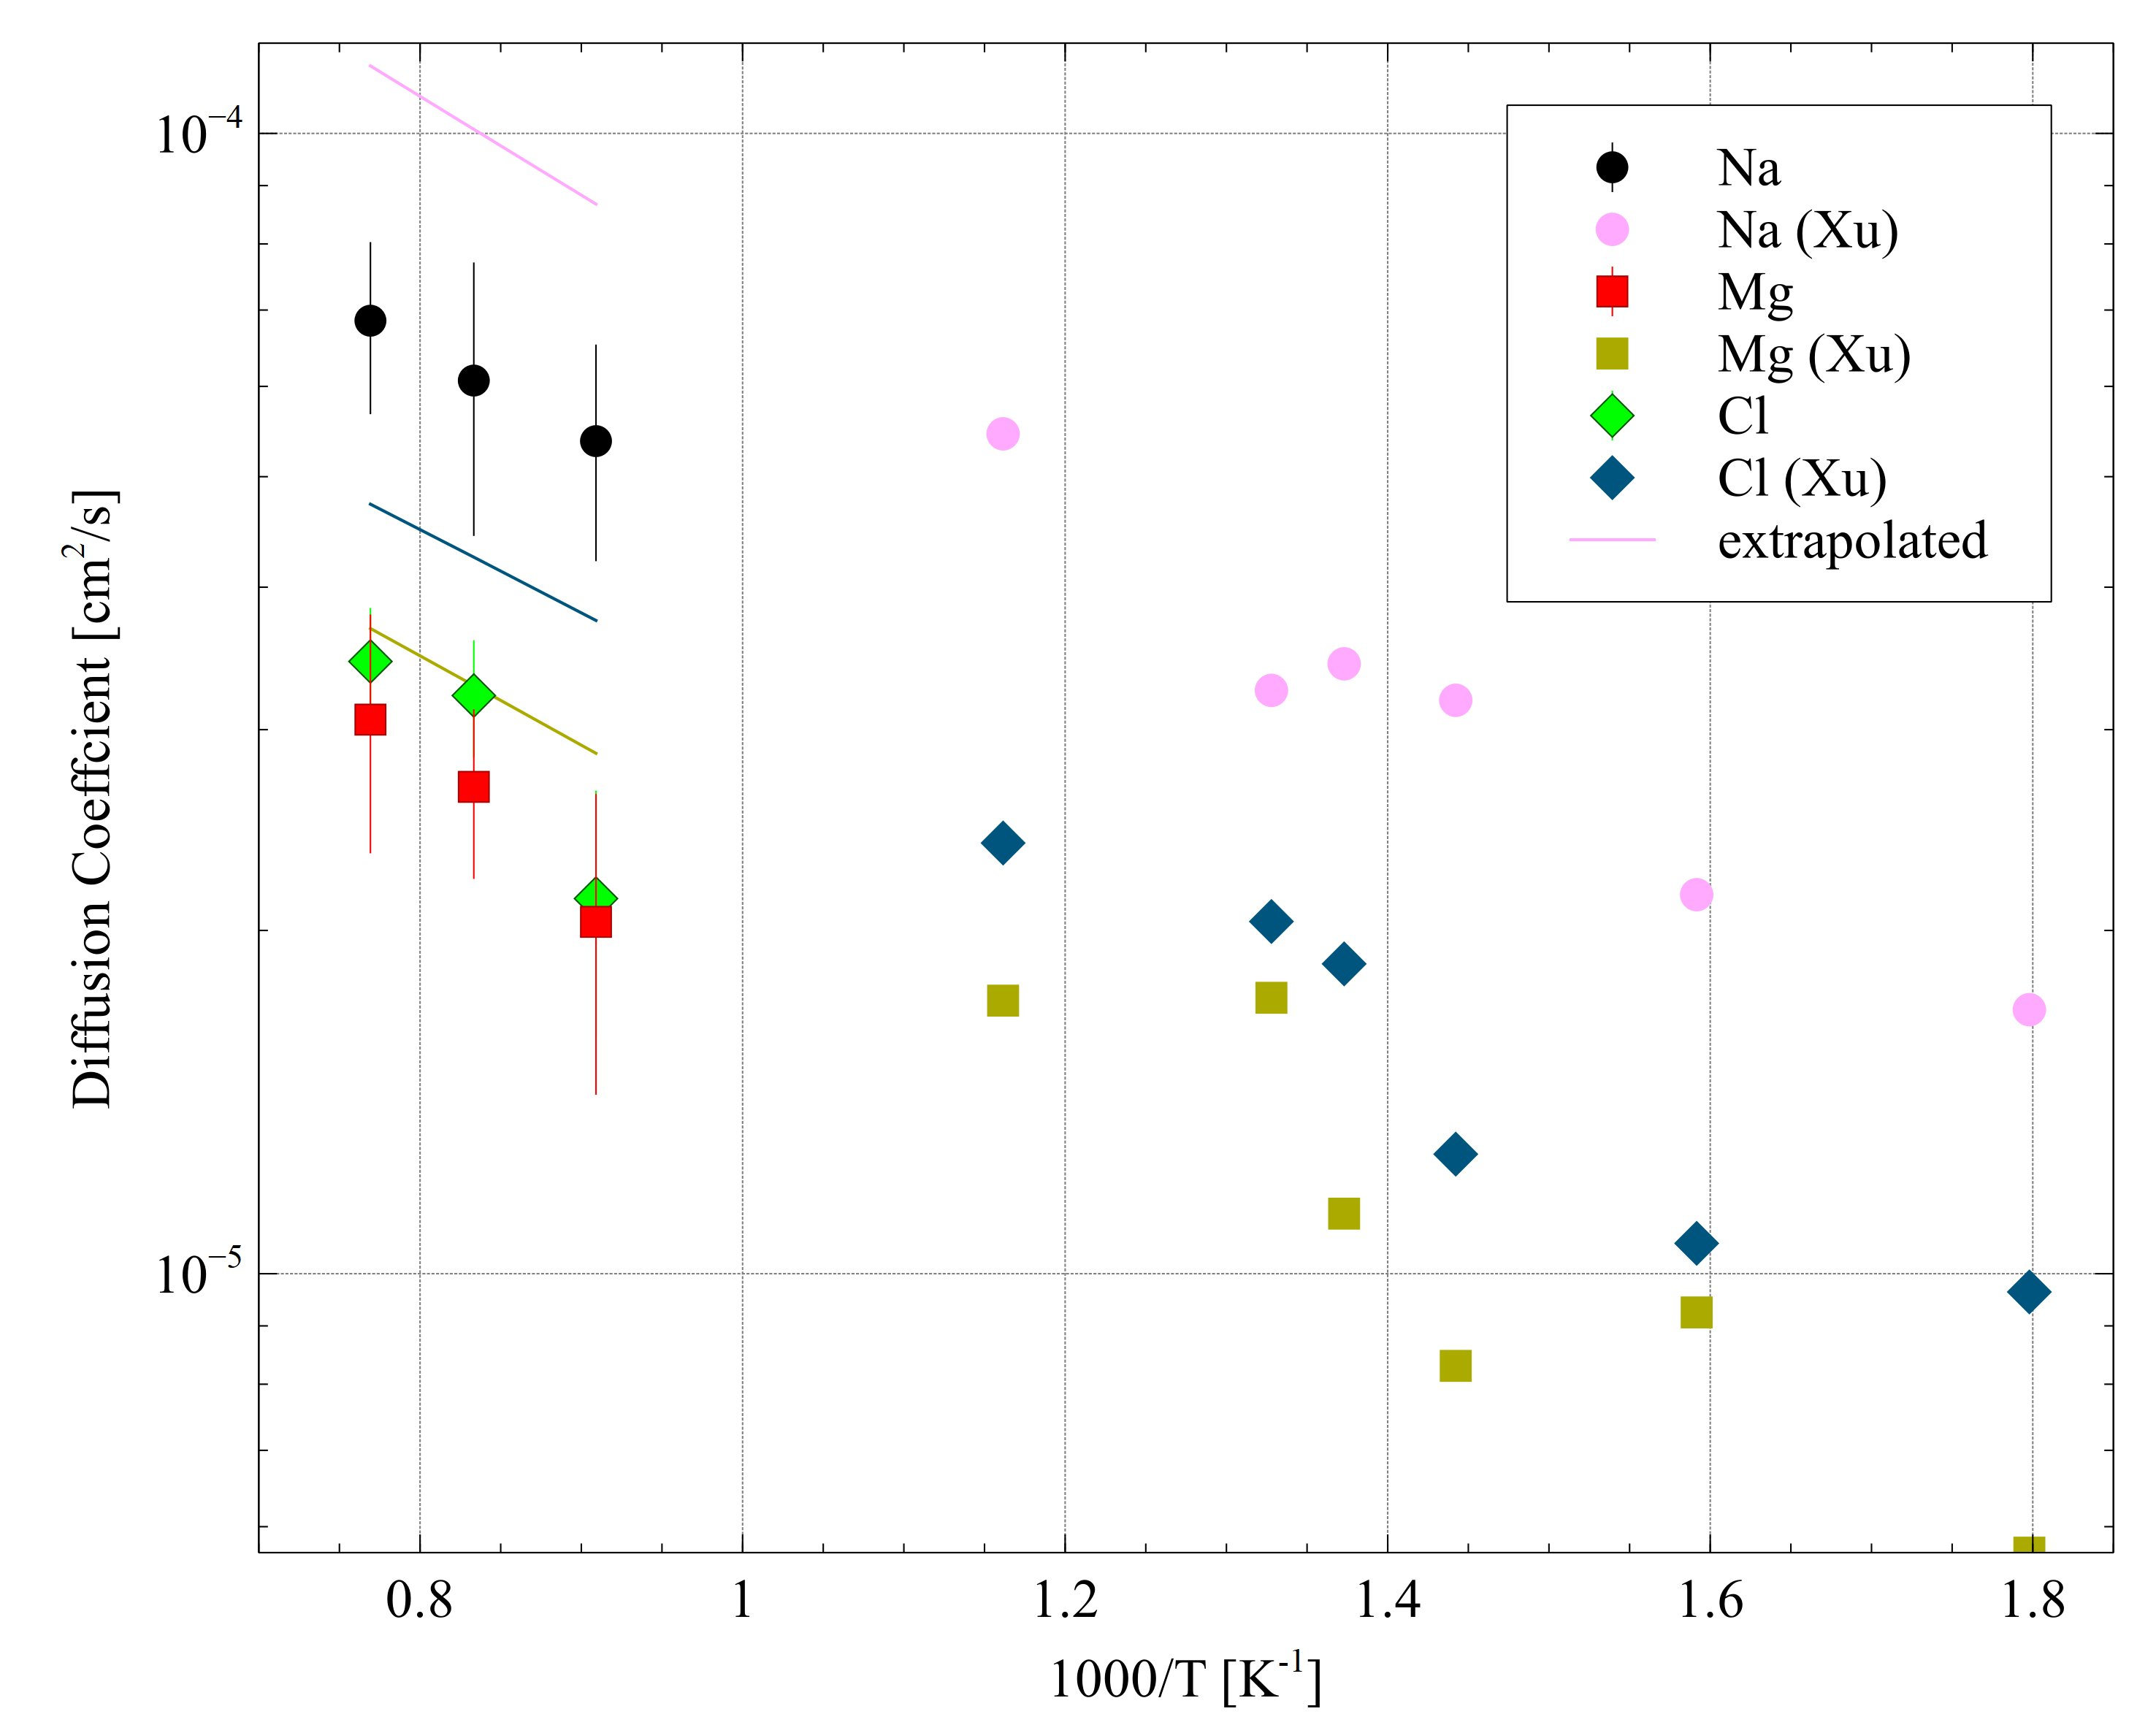
\includegraphics[width=0.7\textwidth]{diff_eutectic_nacl_mgcl2.jpg} 
 \caption{The diffusion coefficient of eutectic NaCl-MgCl$_2$ compared against extrapolated AIMD data by Xu et al. \cite{xu2020powerful}.}
 \label{fig:NaCl-MgCl2-diffuion}
\end{figure} 

 The diffusion coefficient of NaCl and MgCl$_2$ is shown in Fig. \ref{fig:NaCl_and_MgCl2-diffuion}A and \ref{fig:NaCl_and_MgCl2-diffuion}B, respectively. It can be observed that all species in both systems follow an Arrhenius behavior. The diffusion of the Mg and Cl ions in the eutectic composition is faster than in MgCl$_2$, while there is no noticeable change between the Na and Cl ions in NaCl versus the eutectic composition. This makes qualitative sense when considering the network formation of MgCl$_2$ rich salts \cite{LIANG2020}, which one would expect would exhibit slower diffusive properties. For the NaCl system, the Na and Cl ions underestimate the diffusion coefficient when compared to Janz \cite{janz_Diffusion}. There are no available MgCl$_2$ experimental diffusion coefficients available in the literature. Table \ref{table:nacl_and_mgcl2-beta} shows the beta parameters for NaCl and MgCl$_2$ systems, generally showing values above 0.9. 


\begin{figure}[!h]
 \centering
 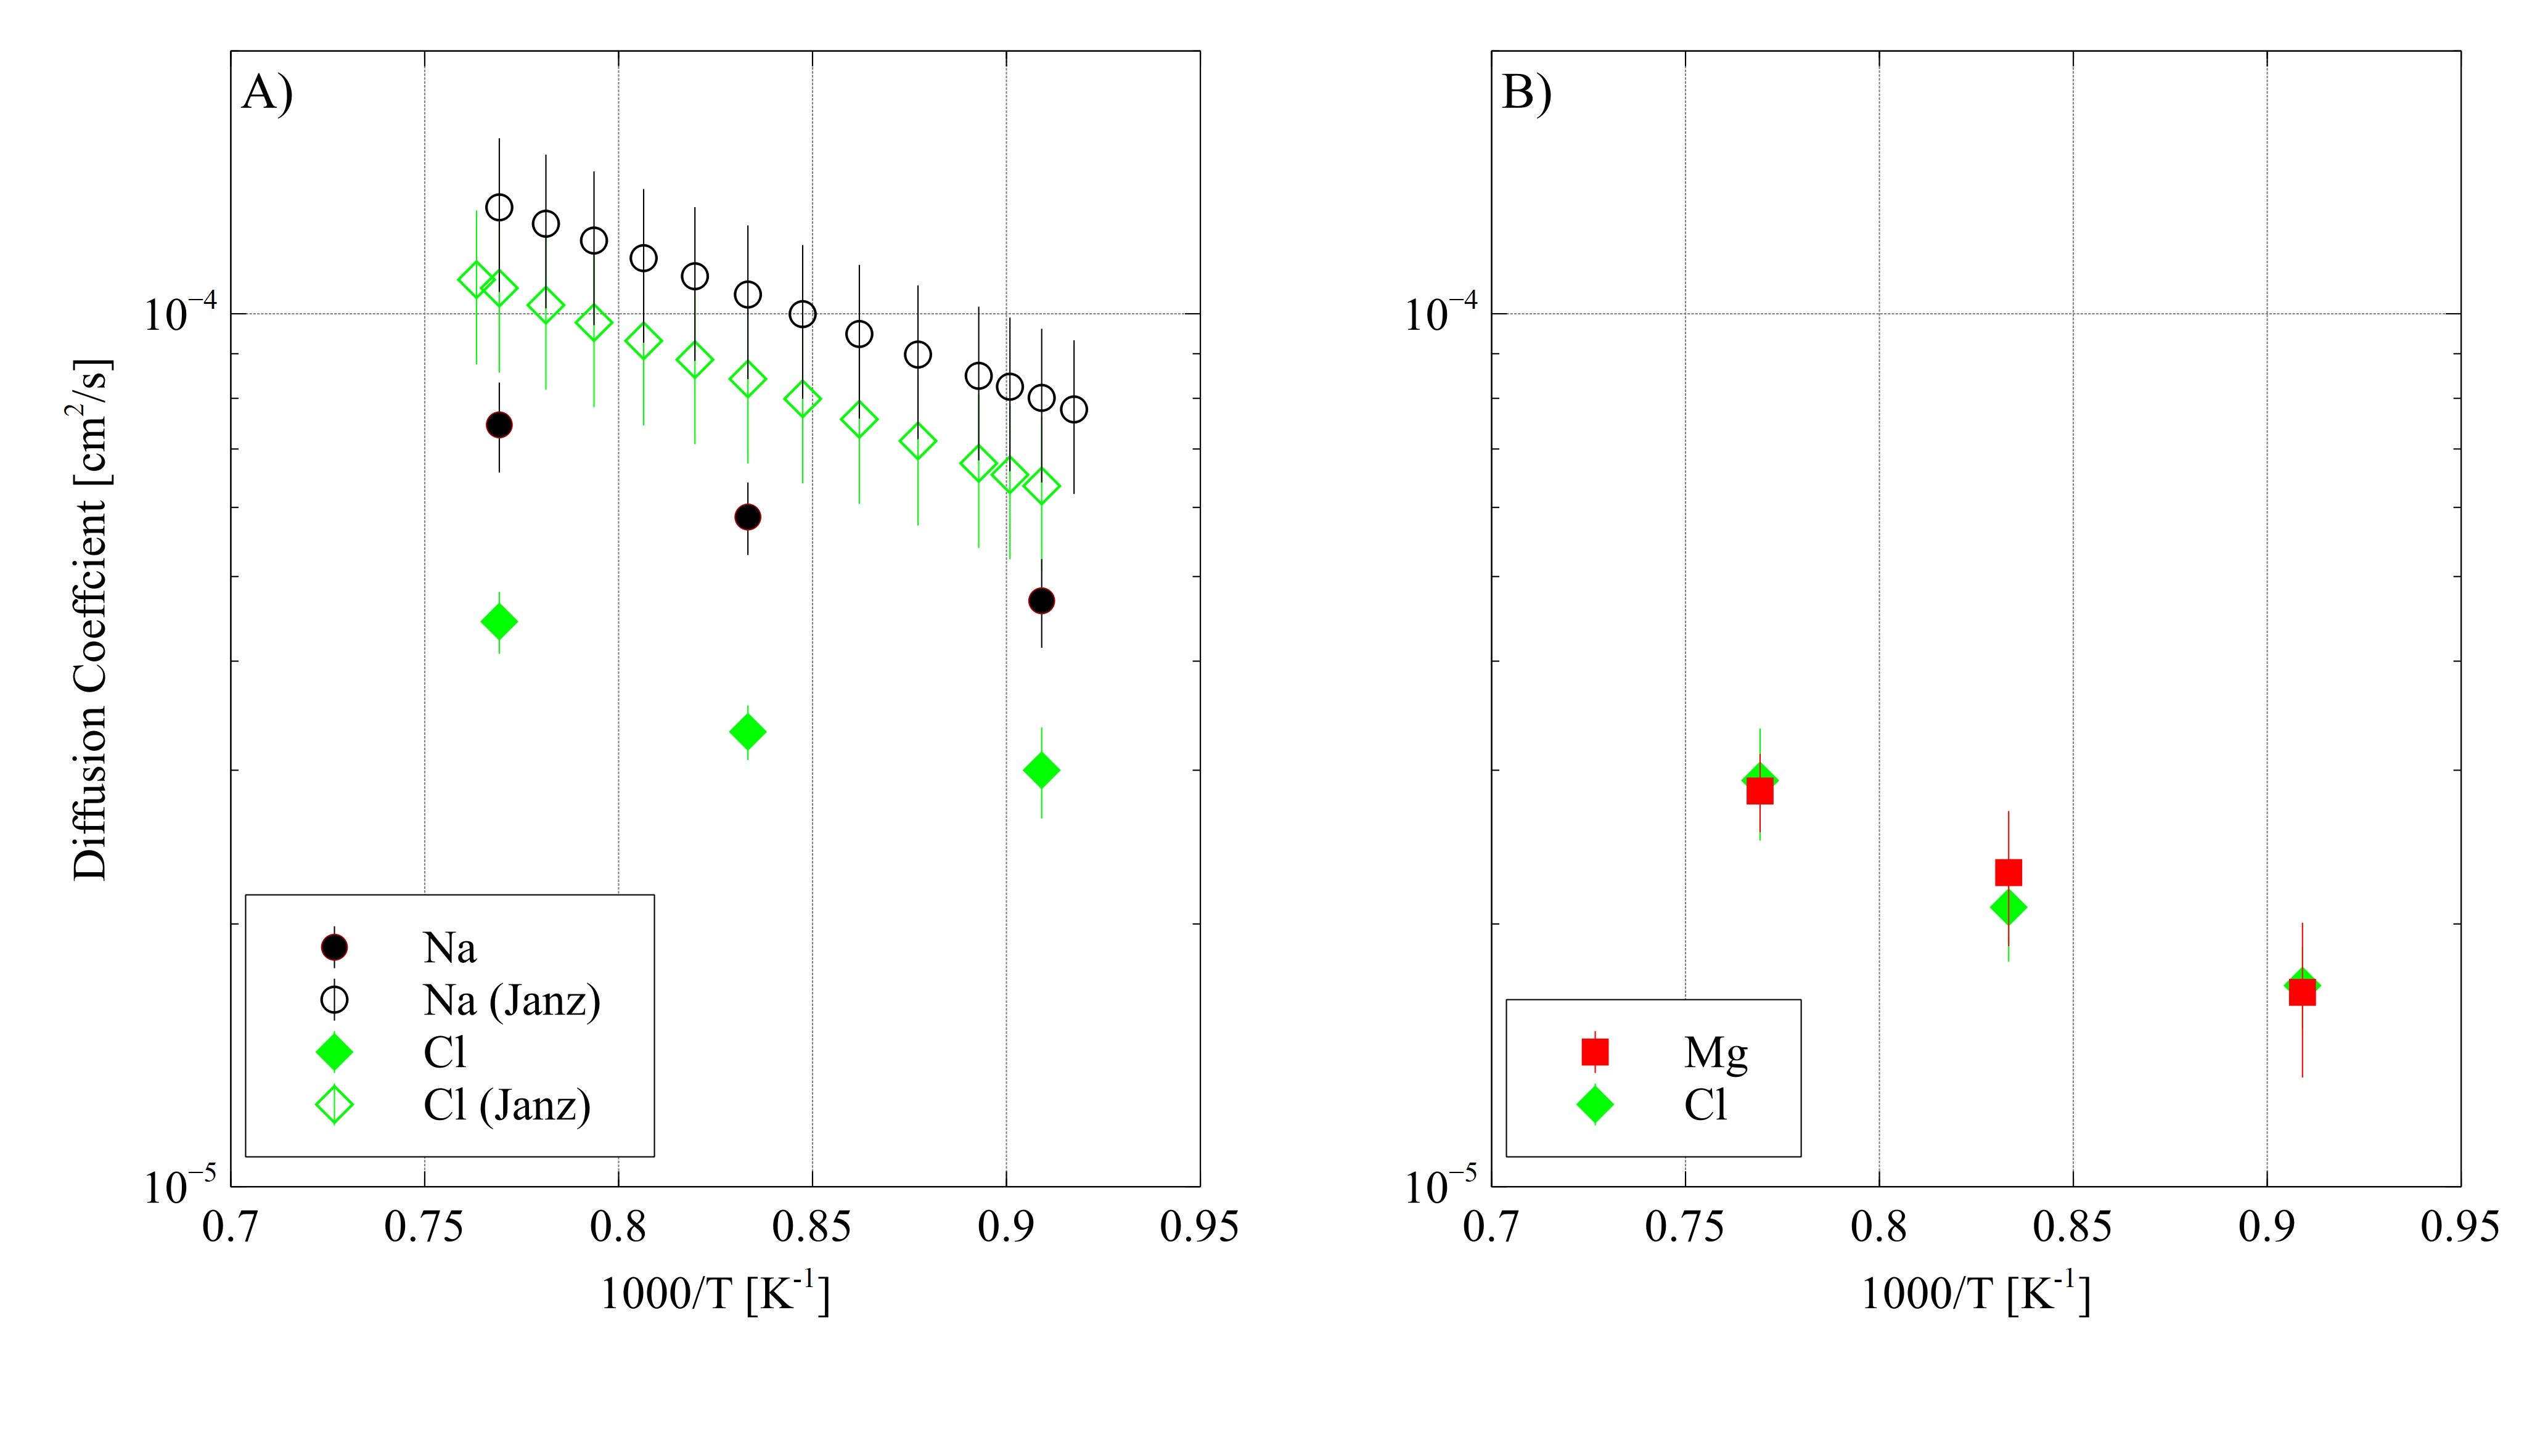
\includegraphics[width=0.9\textwidth]{diff_nacl_and_mgcl2.jpg} 
 \caption{The diffusion coefficient of a) NaCl and b) MgCl$_2$. NaCl is compared against experimental results \cite{janz_Diffusion}. Closed markers are AIMD (this study) and open markers are experimental results.}
 \label{fig:NaCl_and_MgCl2-diffuion}
\end{figure}

The total diffusion coefficient for NaCl, MgCl$_2$, and the eutectic can be seen in Fig. \ref{fig:NaMgCl_total_diff}. NaCl has the fastest diffusion, MgCl$_2$ has the slowest, and the eutectic falls in the middle.
The activation energy and the pre-exponential factor for the diffusion coefficient of the NaCl-MgCl$_2$ system can be seen in Table \ref{table:activation_energy}. The activation energy for the eutectic composition is lower than the endpoint systems. The Na ion activation energy in NaCl is underestimated when compared to Janz \cite{janz_Diffusion} by 8\% while the Cl ion is also underestimated by 17\%. This is a similar level of underestimation to the KCl system. When comparing the total diffusion coefficient of NaCl-MgCl$_2$ eutectic to the value calculated from a linear interpolation of the endpoints, the data generally match very well. Only at 1300K do the error bars not overlap, and Arrhenius fits (not shown) are quite similar. This was not expected, due to the non-linear density variation with composition previously observed in this system \cite{duemmler_naclmgcl}, which indicates non-ideal mixing behaviors. Thus, the assumption of ideal or non-deal mixing behavior of different properties is not always consistent even within a given system. 

\begin{figure}[!h]
 \centering
 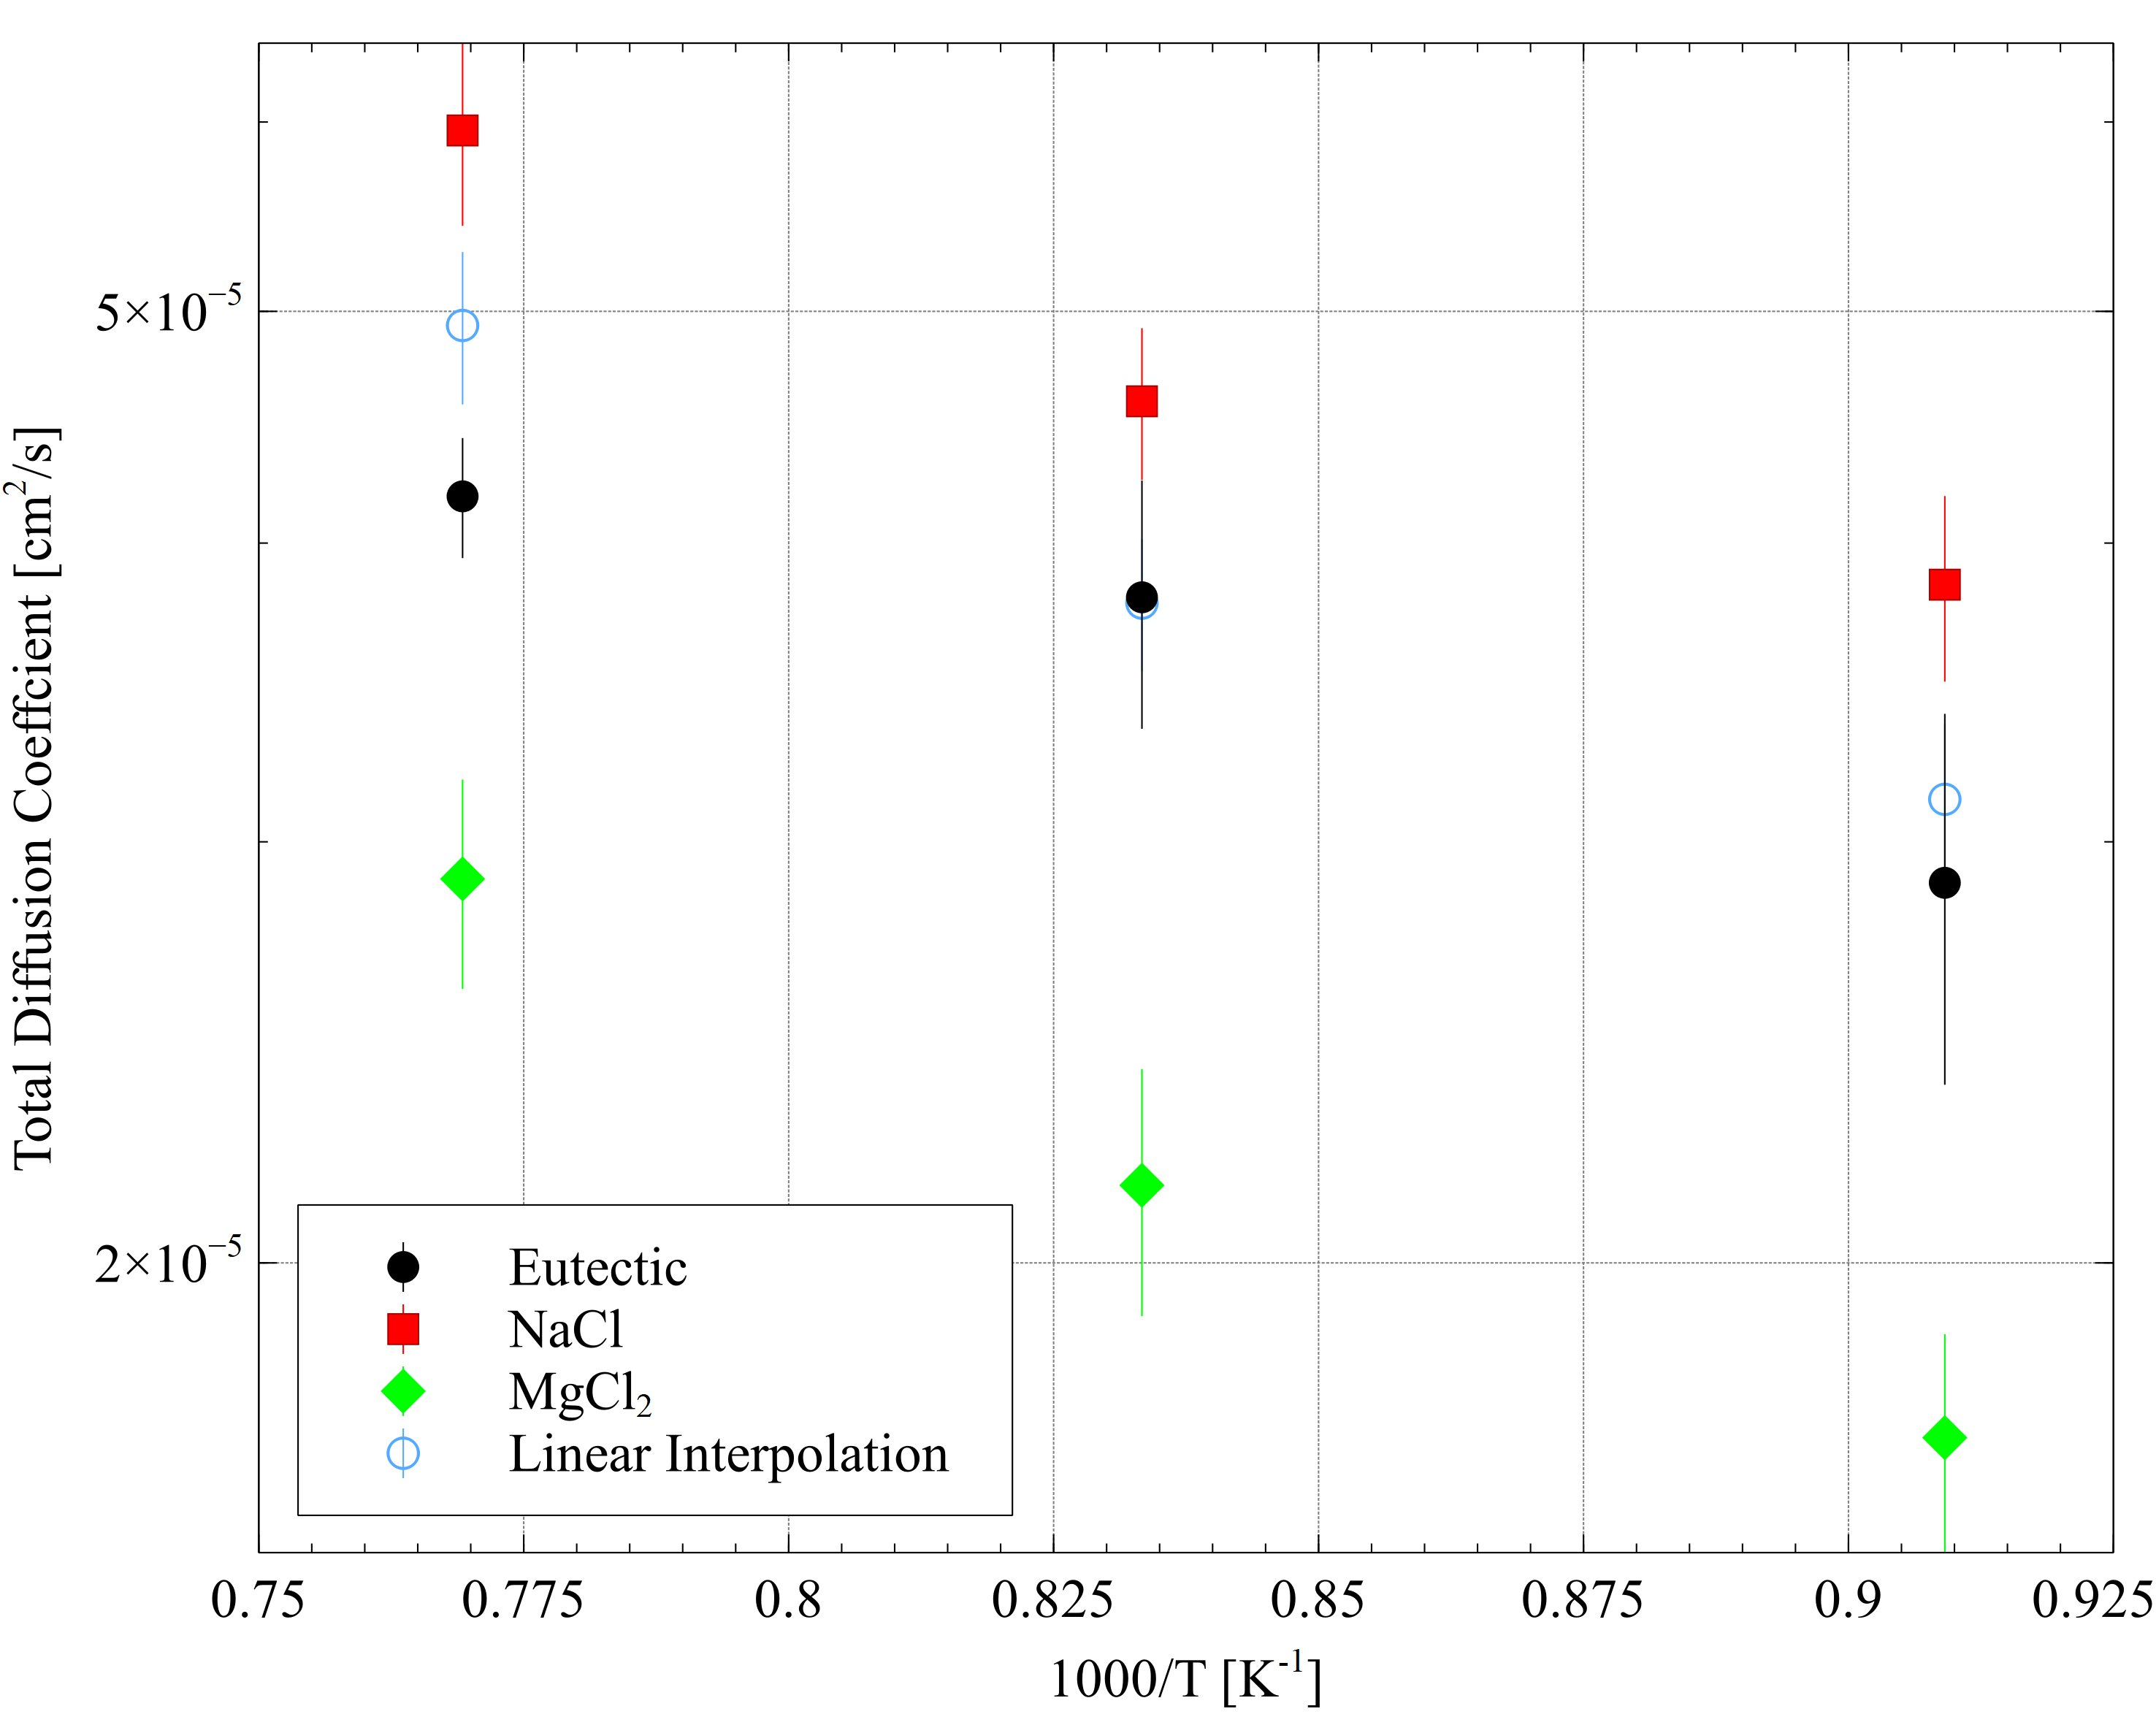
\includegraphics[width=0.7\textwidth]{diff_total_namgcl.jpg} 
 \caption{The total diffusion coefficient of NaCl, MgCl$_2$ and the eutectic. The eutectic is compared to the value calculated via linear interpolation of the endpoints.}
 \label{fig:NaMgCl_total_diff}
\end{figure}
\FloatBarrier



\subsubsection{Viscosity}

The viscosity is calculated via the Stokes-Einstein-Sutherland equation (\cref{eq:SES}) utilizing the solvodynamic radius from Table \ref{Table:solvodynamic}. The viscosity of the NaCl-MgCl$_2$ system can be seen in Fig. \ref{fig:viscNaCl}, which shows that MgCl$_2$ has the largest viscosity while NaCl has the lowest, with the eutectic in the middle. This trend is not observed when compared to the experimental literature \cite{janz_visc,janz_osti,Tasidou} which shows that MgCl$_2$ has the largest, the eutectic has the smallest, and NaCl being slightly larger than the eutectic. The viscosity of MgCl$_2$ and eutectic are overestimated when compared to the experimental values reported by Janz \cite{janz_visc, janz_osti}. However, the viscosity of NaCl agrees well with experimental values reported by Tasidou et al. \cite{Tasidou} and Janz et al. \cite{janz_osti}. 
\begin{figure}[h!]
 \centering
 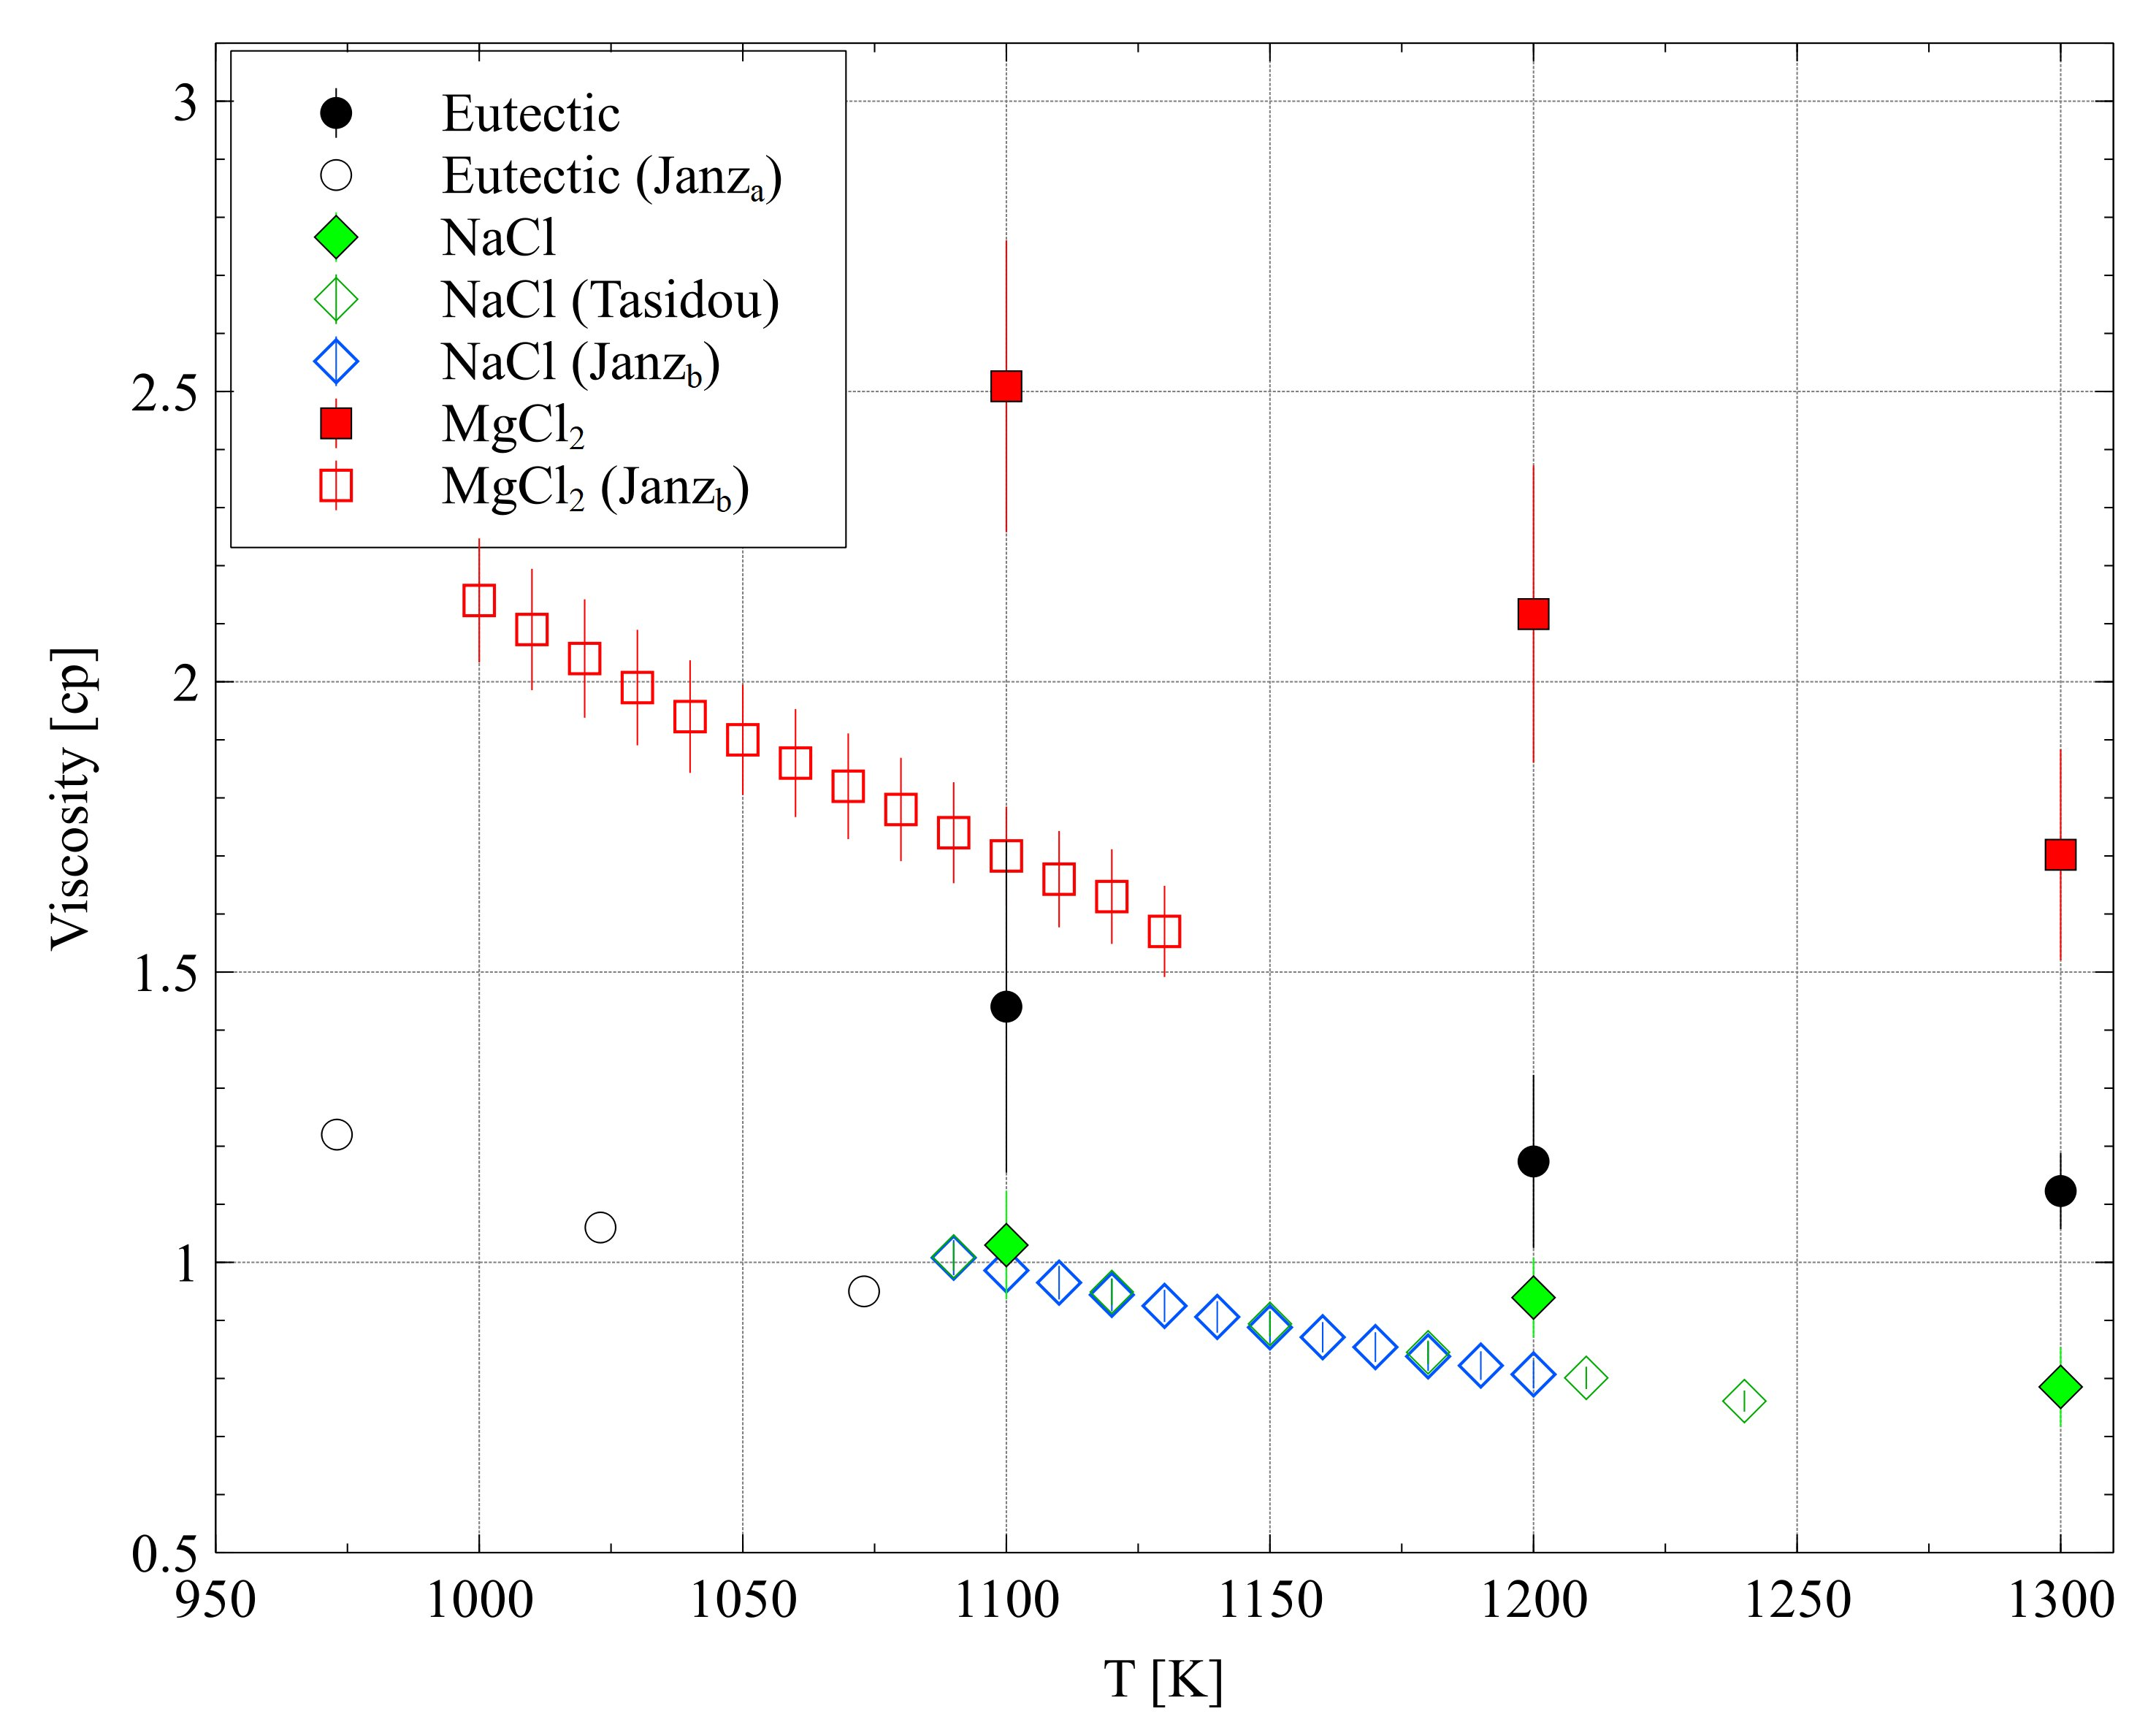
\includegraphics[width=0.7\textwidth]{visc_nacl-mgcl2.jpg} 
 \caption{The viscosity of the NaCl-MgCl$_2$ eutectic, NaCl, and MgCl$_2$ systems. Solid markers are this study and the open markers are experimental studies \cite{janz_visc,Tasidou,janz_osti}.}
 \label{fig:viscNaCl}
\end{figure} 

\subsubsection{Heat Capacity}
The isochoric and isobaric heat capacities of the NaCl-MgCl$_2$ systems can be seen in Fig. \ref{fig:nacl-mgcl2 cv}. Only the eutectic composition displays a $C_V$ with a statistically significant (negative) dependence upon the temperature, while the separate salt components are effectively constant with temperature. An observable trend is the ordering of the magnitude of the heat capacity for each system, where the lowest is NaCl, followed by the eutectic, and the highest $C_V$ for the MgCl$_2$ system. This trend is also seen in the calculated $C_P$ values. The calculated $C_P$ values use \textit{$\alpha$} and \textit{$\beta_T$} values from our previous work on NaCl-MgCl$_2$ systems \cite{duemmler_naclmgcl}. Both $C_P$ and $C_V$ for MgCl$_2$ share the same trends of remaining constant over the studied temperature range. For the NaCl system, both the calculated $C_P$ and the $C_V$ are also constant over temperature, while the experimental data reported by Janz shows a decreasing trend with increasing temperature. However, the rate of decrease shown in Janz's work falls within the error bars of our reported data, and thus the presence of a trend is indistinguishable. Importantly, the magnitude of the $C_P$ for NaCl from this work matches quite well with the experimental literature. For the eutectic composition, there are no experimental values for either $C_P$ or $C_V$ so they are compared to the available computational literature. $C_P$ values are reported for the eutectic composition in our previous work \cite{duemmler_naclmgcl} and in Xu et al.\cite{xu2020powerful}. In our previous work, the temperature range studied was 800 - 1300 K which showed a constant value of 74.96 J/mol-K for $C_P$. Xu et al. studied a lower temperature range (728 - 861 K) with values ranging from 352 to 428 J/mol-K which drastically overestimates the endpoints reported in Janz, this work, and our previous work, so it is not considered here. When we compare the $C_P$ calculated here to the value reported in previous work, we see good agreement at the higher temperatures. While this work shows a negative correlation with temperature for the eutectic $C_P$, our previous computational study showed no variation with temperature. However, uncertainties associated with both the methods presented here and the methods in our previous work make it difficult to discern if there is a statistically significant trend with temperature.


\begin{figure}[h!]
 \centering
 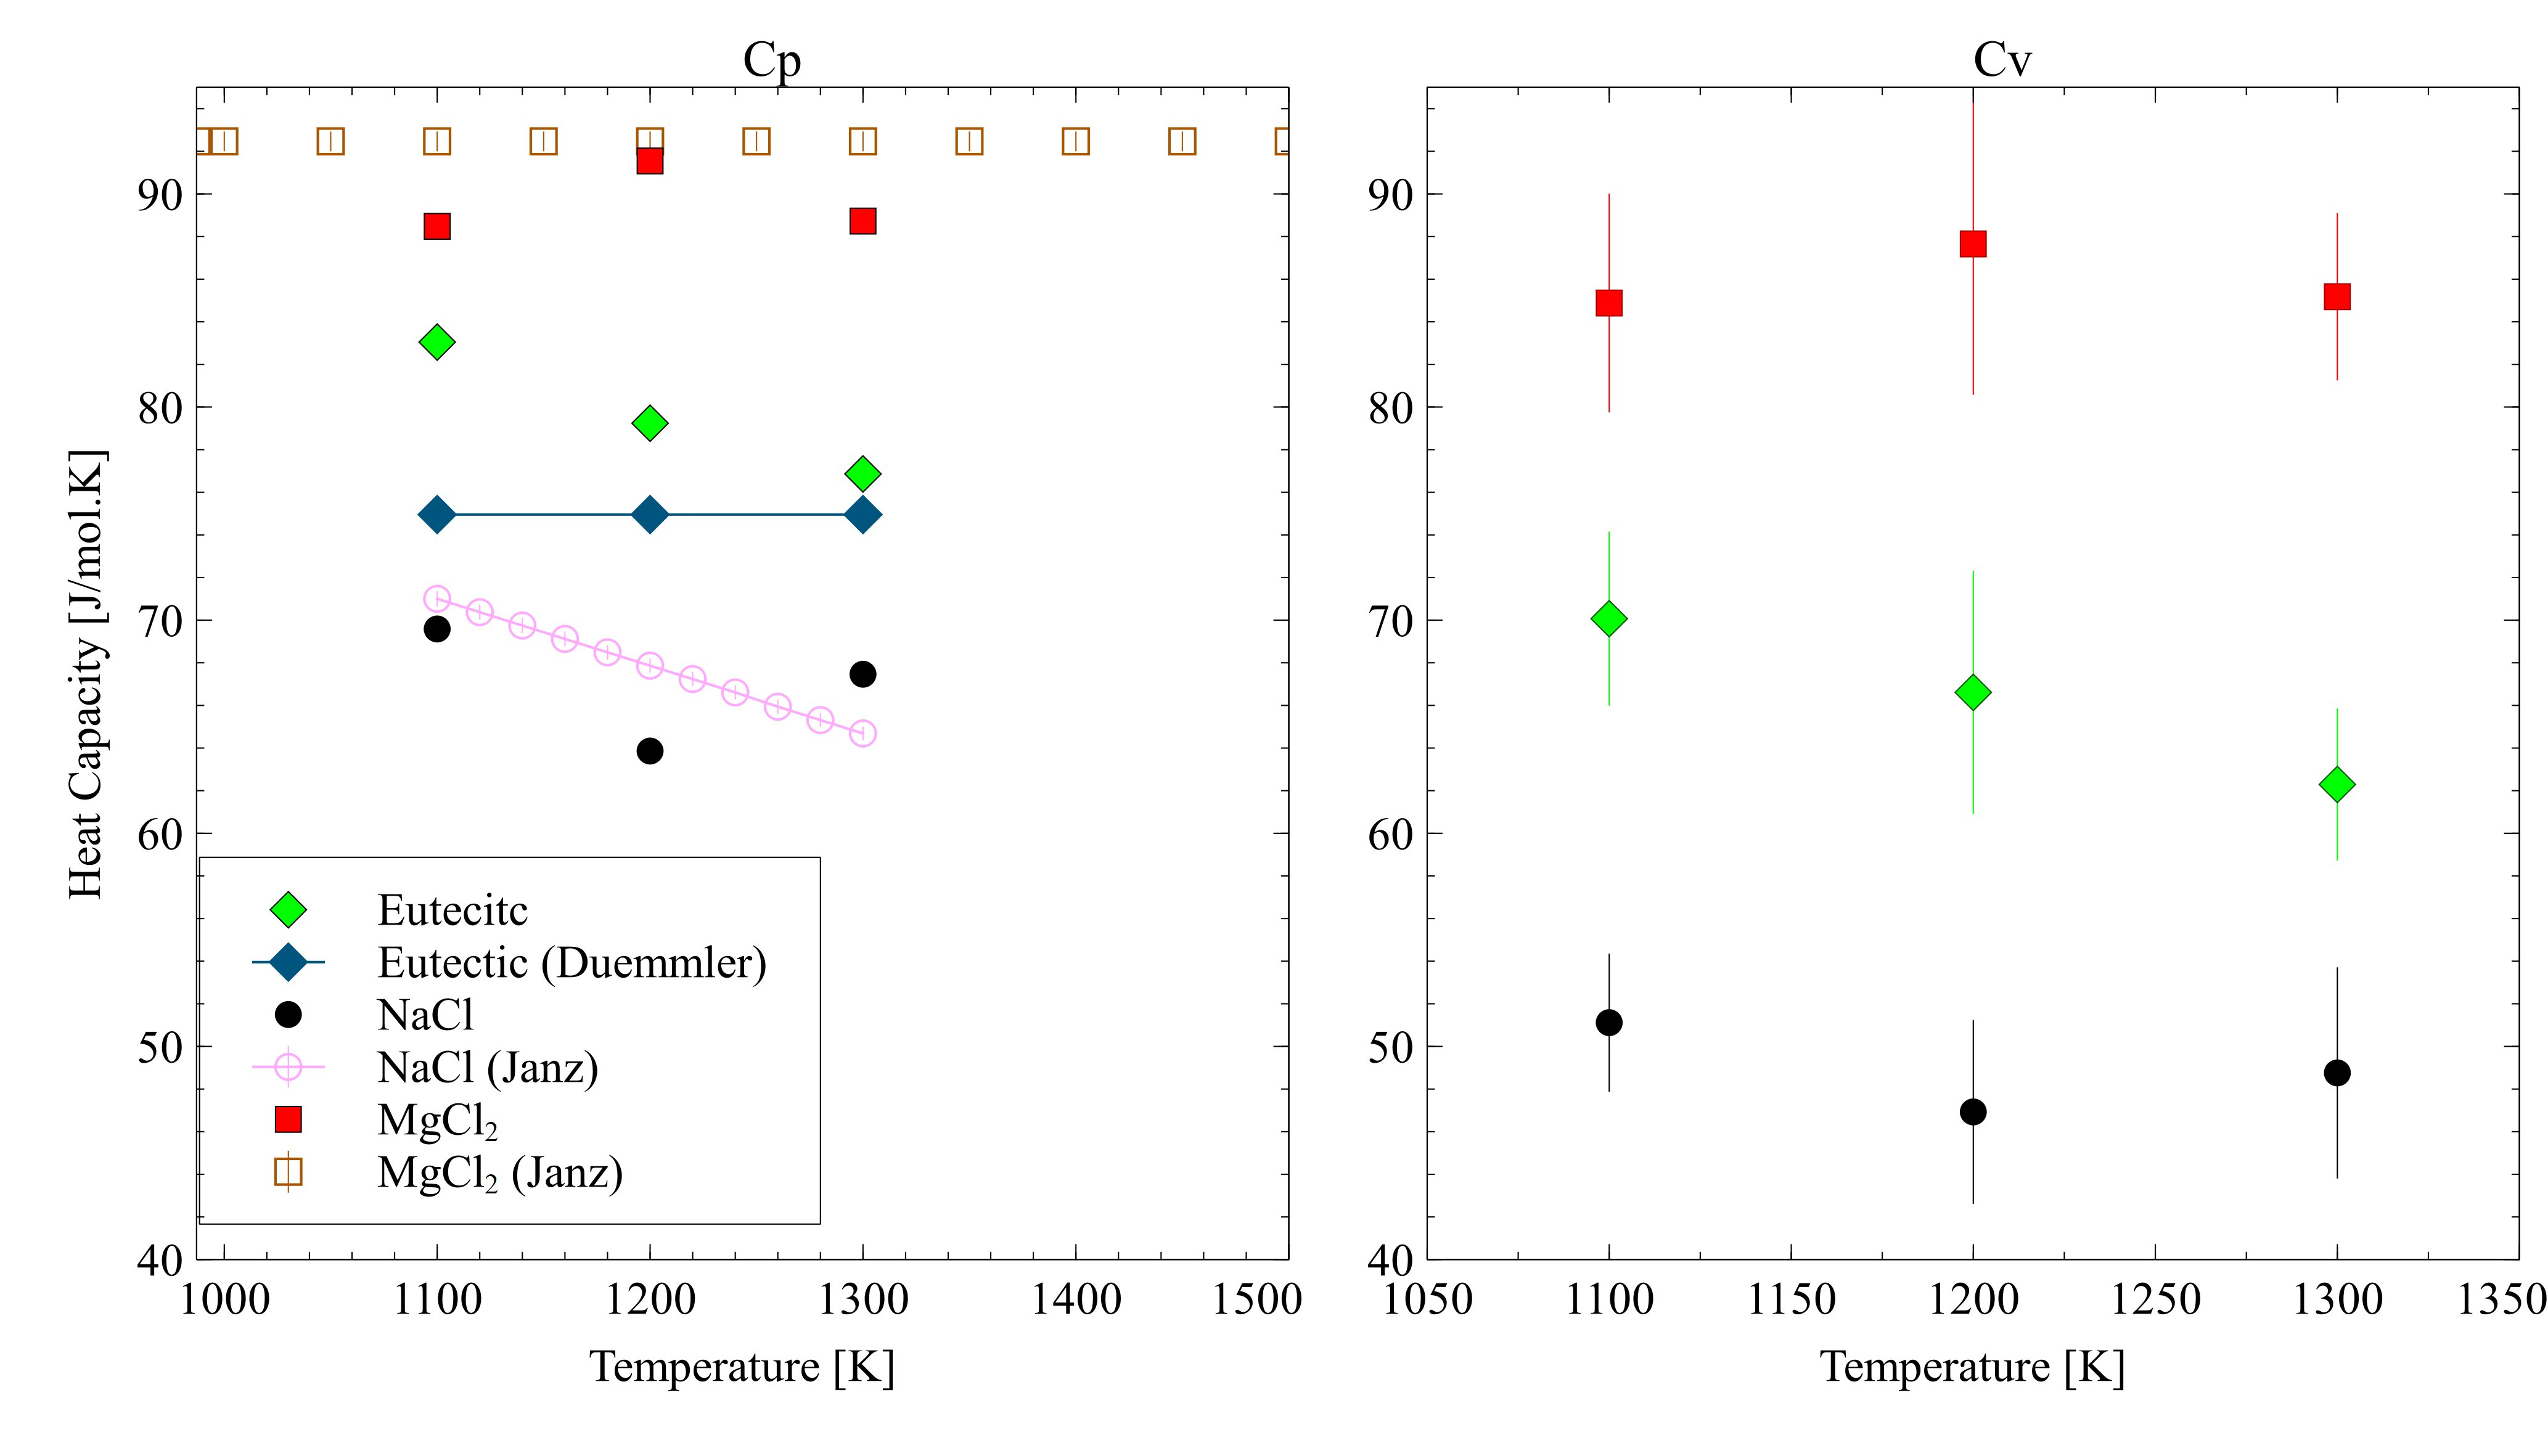
\includegraphics[width=0.9\textwidth]{cv_nacl-mgcl2.jpg} 
 \caption{Both the isobaric and isochoric heat capacities for NaCl-MgCl$_2$ eutectic, NaCl, and MgCl$_2$ systems. The isobaric heat capacity is compared against experimental $C_P$ values from \cite{janz_osti} and an AIMD study from Duemmler et al. \cite{duemmler_naclmgcl}. Closed markers are computational results and open markers are experimental values.}
 \label{fig:nacl-mgcl2 cv}
\end{figure} 

 
\FloatBarrier

\section{Discussion}

\subsection{Comparison to Literature}

Given that there are relatively few experimental results, and the majority were conducted prior to 1980, it can be instructive to analyze the consistency of experimental data to provide a baseline for comparison to the computational results. There is generally good agreement among the experimental results for LiCl-KCl, especially for viscosity (Fig. \ref{fig:LiCl-KCl visc}) which includes both older studies (Brockner-1975 \cite{brockner1975high} and Janz-1975 \cite{janz_visc}) and newer studies (Tasidou-2019 \cite{Tasidou}). There are an insufficient number of studies on the NaCl-MgCl$_2$ system to construct a comparison and identify consistency in the literature. Additionally, there are substantial error bars on a variety of experimental quantities which serve as a basis for comparison in this work, and further experimental evaluation of thermophysical and transport properties at selected compositions and temperatures is warranted to increase the certainty of the existing experimental data.

There are significant differences when comparing AIMD results from this work to Bengston \cite{Bengston2014}, which tended to have larger values for the diffusivity of LiCl-KCl than reported here. As mentioned before there are several major differences between this study and the one conducted by Bengston et al. \cite{Bengston2014} including the dispersion correction method, simulation size, and simulation time. The dispersion correction used by Bengston et al. was the DFT-D2\cite{grimme} while this work used the vdW-DF2 \cite{Dion2004}. In our prior work \cite{duemmler_liclkcl}, we evaluated the relative accuracy of a variety of dispersion formalisms for the description of the LiCl-KCl system. However, the D2 formalism was not included in this evaluation, but an updated version, the DFT-D3 method, was tested. What was determined is that while the DFT-D3 dispersion formalism yielded the least total error in predictions of the density, the vdW-DF2 formalism predicts the correct experimental trend of the density with composition, and thus was deemed superior. Additionally, the time increment and total time also differed between the studies. This work shows that the 12 ps simulations used in Bengston's study do not account for time-dependent behaviors, which could explain some of the differences between this study and theirs. Further, the 12 ps segments used in Bengston's study were subdivided into four sub-blocks which shortens the actual trajectory even further.Another difference is the method used to calculate the diffusion coefficient. In this work, the msd trajectory is used to calculate the diffusion coefficient via Eq. \ref{eq:Einstein} for 6 unique trajectories and then averaged for the final value with the error shown as the standard deviation of those 6 simulations. In Bengston's study, they used a slightly different method to calculate the msd. Their method allowed the shifting of the time origin point. They broke their ~12 ps simulation into 4 blocks where each block had a calculated diffusion coefficient with the number of time origins equaling half the block size \cite{Bengston2014}. They note that the selection of time origins is to ensure equal-length trajectories. Following the calculation of the diffusion coefficient of each block they would then average that for their final diffusion coefficient. We utilized a single time origin and a significantly longer simulation time to ensure that any time-dependent behaviors were captured. The method of Bengston would only capture behaviors which occur on a roughly 4 ps timescale. Regretfully, there are no other computational studies exploring transport phenomena in these molten salts from an AIMD perspective.

When comparing the computational data to the experimental data, there is often reasonable, if imperfect, agreement. The numerical error between the computation results and the experimental equivalent varied from within the experimental error to 30\% difference. While this numerical error can be somewhat large for certain properties, the temperature and compositional trends agreed with the experimental results. The actual trends can be as important when creating safety margins for nuclear reactors. The numerical uncertainty can be accounted for but the correct trends are required for any safety margin to be accurate or reasonable.

\subsection{LiCl-KCl versus NaCl-MgCl$_2$}

The total diffusion coefficient for the LiCl-KCl system and the NaCl-MgCl$_2$ system can be seen in Fig. \ref{fig:likcl_total_diff} and Fig. \ref{fig:NaMgCl_total_diff}, respectively. The eutectic LiCl-KCl system diffuses faster than eutectic NaCl-MgCl$_2$ at all temperatures. For the endpoints, LiCl has the fastest diffusion followed by KCl and NaCl, with MgCl$_2$ being the slowest. The total diffusion for eutectic LiCl-KCl has a value outside the standard deviation of the linearly interpolated diffusion coefficient calculated from LiCl and KCl total diffusion values. This is not a trait shown in eutectic NaCl-MgCl$_2$ which only has a single value at 1300 K that does not overlap with the standard deviation of the linearly interpolated diffusion coefficient. The eutectic NaCl-MgCl$_2$ total diffusion coefficient can be approximated with linear interpolation while the eutectic LiCl-KCl cannot.


When comparing the heat capacity ratio or adiabatic index ($C_P$/$C_V$) for the eutectic LiCl-KCl system to the eutectic NaCl-MgCl$_2$ system, the former has a larger value with a range from 1.22 to 1.28 compared to 1.19 to 1.23 of the latter. MgCl$_2$ is the system with the lowest adiabatic index with a value of 1.04 for all temperatures. NaCl is the system with the largest adiabatic index with a range of 1.36 to 1.38. The LiCl and KCl have values ranging from 1.21-1.27 and 1.33-1.35, respectively. In both systems, the eutectic system has an adiabatic index that falls in the middle of their respective endpoint salt values. The heat capacity ($C_P$ or $C_V$) can be accurately predicted through the use of AIMD for both the LiCl-KCl system and the NaCl-MgCl$_2$ system.

\subsection{Outlook}
Calculating the transport properties of molten salts through AIMD methods comes with a set of drawbacks. The most obvious aspect is related to the computational expense, which limits the ability to reduce scatter in the data through the use of larger systems or conducting longer simulations. Extending simulations to the nanosecond scale for systems of over 1000 atoms remains strictly in the realm of classical molecular dynamics. This work has conducted extensive convergence testing to determine the minimum simulation size of 100 atoms and simulation length of 50 ps increments is needed for the reliable calculation of the molten salt transport properties. This study has been shown that it is possible to extract transport properties that reasonably compare to the experimental values, and the simulations from which those transport properties have been derived have reached a truly diffusive regime. Thus, AIMD is a valid method for calculating the transport properties of unstudied molten salts, particularly with the ability to explore arbitrary compositions and temperatures, without the requirement for the development of an interatomic potential. 

\FloatBarrier
\section{Conclusions}
This work has shown that a system with 100 atoms has comparable results for the transport properties when compared with a 200 atom system, for these specific salt systems. This work also shows that a minimum time increment of 50 ps should be used for the calculations of transport properties and a total simulation time of 300 ps has reasonable agreement with the literature. The diffusion coefficient, viscosity, activation energy and pre-exponential factor of the diffusion coefficient, and both isochoric and isobaric heat capacity were calculated for LiCl, KCl, eutectic LiCl-KCl, NaCl, MgCl$_2$, and eutectic NaCl-MgCl$_2$. For LiCl, NaCl, and KCl the diffusion coefficient values calculated through AIMD underestimate the experimental results. The diffusion coefficient calculations for the LiCl-KCl eutectic estimate a lower value than another AIMD study, while the diffusion coefficient of eutectic NaCl-MgCl$_2$ shows lower values than the extrapolations of an AIMD study. There is good agreement with the literature for the viscosity of KCl and NaCl, while the predicted values for eutectic LiCl-KCl underestimate the experimental results. The calculated viscosity for eutectic NaCl-MgCl$_2$ and MgCl$_2$ overestimates the experimental results. There is good agreement with the literature for the isobaric heat capacity for all systems. This work shows that AIMD is capable of accurately calculating the transport properties of molten salts and capturing any present time-dependent behaviors. This was the first work to extend AIMD time scales beyond 200 ps to explore the transport properties of molten salts.

\section{Acknowledgements}

This material is based upon work supported under a University Nuclear Leadership Program Graduate Fellowship. This work is also supported through the INL Laboratory Directed Research and Development (LDRD) Program under DOE Idaho Operations Office Contract DE-AC07-05ID14517. This research made use of the resources of the High-Performance Computing Center at Idaho National Laboratory, which is supported by the Office of Nuclear Energy of the U.S. Department of Energy and the Nuclear Science User Facilities.  
\FloatBarrier

\appendix

\section{}
\subsection{Diffusion coefficient}
The diffusion coefficient for LiCl-KCl eutectic at 1200 K run in parallel or sequential simulations can be seen in Table\ref{Table:parVSseq}.

\begin{table}[h]
\centering
\caption{The diffusion coefficient [10$^5$*cm$^2$/s] for 100 atoms parallel vs sequential convergence study. }
\begin{tabular}{lllll}
\hline
Simulation Increment   {[}ps{]} & Type       & Li       & K        & Cl       \\
\hline
25                              & parallel   & 9.89 $\pm$ 1.73& 6.70 $\pm$ 0.960& 5.38 $\pm$ 1.05\\
& sequential & 9.99 & 6.97 & 5.43 \\
50 & parallel   & 7.85  $\pm$ 1.14& 6.75 $\pm$ 1.38& 5.56 $\pm$  0.640\\
 & sequential & 9.58 & 5.40 & 5.97 \\
100 & parallel   & 10.1  $\pm$ 1.20& 6.39 $\pm$  0.01 & 6.16 $\pm$  0.15\\
& sequential & 9.93 & 6.82 & 6.57 \\
\hline
\end{tabular}
\label{Table:parVSseq}
\end{table}
\FloatBarrier

The tabulated diffusion coefficient for LiCl-KCl eutectic can be seen in Table \ref{Table: licl-kcl-eut diffusion}.

\begin{table}[h]
\centering
\caption{The diffusion coefficient of the LiCl-KCl eutectic system with the standard deviation with units of 10$^5$ cm$^2$/s }
\begin{tabular}{lllll}
\hline
T(K) & K           & Li          & Cl          &  \\
\hline
1300 & 7.59$\pm$1.98 & 11.89$\pm$1.91 & 6.94$\pm$0.84 &  \\
1200 & 8.34$\pm$2.23 & 9.33$\pm$1.40  & 5.78$\pm$0.58 &  \\
1100 & 5.85$\pm$1.43 & 7.87$\pm$1.90  & 4.64$\pm$0.36 &  \\
1000 & 4.52$\pm$1.16 & 6.53$\pm$1.34  & 3.54$\pm$0.53 &  \\
900  & 3.44$\pm$0.83 & 5.28$\pm$1.22  & 2.73$\pm$0.54 &  \\
800  & 2.17$\pm$0.60 & 2.97$\pm$0.36  & 1.62$\pm$0.32 &  \\
700  & 1.71$\pm$0.48 & 2.18$\pm$0.62  & 1.06$\pm$0.23  \\
\hline
\end{tabular}
\label{Table: licl-kcl-eut diffusion}
\end{table}
\FloatBarrier

The tabulated diffusion coefficient for LiCl and KCl can be seen in Table \ref{Table: licl diffusion} and Table \ref{Table: kcl diffusion}.

\begin{table}[h]
\centering
\caption{The diffusion coefficient of the LiCl system with the standard deviation with units of 10$^5$ cm$^2$/s }
\begin{tabular}{lll}
\hline
T(K) & Li           & Cl        \\
\hline
1300 & 20.01 $\pm$2.52 & 7.47 $\pm$1.50  \\
1200 & 14.93 $\pm$1.50  & 6.05 $\pm$0.93 \\
1100 & 13.78 $\pm$1.96& 5.39 $\pm$0.79 \\
\hline
\end{tabular}
\label{Table: licl diffusion}
\end{table}


\begin{table}[h]
\centering
\caption{The diffusion coefficient of the KCl system with the standard deviation with units of 10$^5$ cm$^2$/s }
\begin{tabular}{lll}
\hline
T(K) & K         & Cl        \\
\hline
1300 & 7.17$\pm$0.89 & 6.53$\pm$0.81 \\
1200 & 5.15$\pm$1.02 & 5.73$\pm$1.41 \\
1100 & 4.27$\pm$0.65 & 4.5$\pm$0.64 \\
\hline
\end{tabular}
\label{Table: kcl diffusion}
\end{table}
\FloatBarrier

The tabulated diffusion coefficient for the NaCl-MgCl$_2$ system can be seen in Table \ref{Table: nacl-mgcl2_eut diffusion}.

\begin{table}[h]
\centering
\caption{The diffusion coefficient of the NaCl-MgCl$_2$ eutectic system with the standard deviation with units of 10$^5$ cm$^2$/s }
\begin{tabular}{llll}
\hline
T(K) & Na          & Mg          & Cl          \\
\hline
1300 & 6.85 $\pm$ 1.18 & 3.06 $\pm$ 0.72 & 3.44 $\pm$ 0.39 \\
1200 & 6.07 $\pm$ 1.63 & 2.67 $\pm$ 0.45 & 3.21 $\pm$ 0.38 \\
1100 & 5.37 $\pm$ 1.16 & 2.03 $\pm$ 0.6  & 2.13 $\pm$ 0.52 \\
\hline
\end{tabular}
\label{Table: nacl-mgcl2_eut diffusion}
\end{table}
\FloatBarrier

The tabulated diffusion coefficient for NaCl and MgCl$_2$ can be seen in Table \ref{Table: nacl diffusion} and Table \ref{Table: mgcl2 diffusion}.

\begin{table}[h!]
\centering
\caption{The diffusion coefficient of the NaCl system with the standard deviation with units of 10$^5$ cm$^2$/s }
\begin{tabular}{lll}
\hline
T(K) & Na          & Cl                   \\
\hline
1300 & 7.46 $\pm$ 0.88 & 4.44 $\pm$ 0.36\\
1200 & 5.85 $\pm$ 0.56 & 3.32 $\pm$ 0.24  \\
1100 & 4.69 $\pm$ 0.55 & 3 $\pm$ 0.36     \\
\hline
\end{tabular}
\label{Table: nacl diffusion}
\end{table}

\begin{table}[h!]
\centering
\caption{The diffusion coefficient of the MgCl$_2$ system with the standard deviation with units of 10$^5$ cm$^2$/s }
\begin{tabular}{lll}
\hline
T(K) & Mg          & Cl                \\
\hline
1300 & 2.84 $\pm$ 0.29 & 2.92 $\pm$ 0.43  \\
1200 & 2.29 $\pm$ 0.4  & 2.09 $\pm$ 0.28  \\
1100 & 1.67 $\pm$ 0.34 & 1.7 $\pm$ 0.18   \\
\hline
\end{tabular}
\label{Table: mgcl2 diffusion}
\end{table}
\FloatBarrier

\subsection{Beta parameter}
Table \ref{table:licl-kcl-beta} shows the tabulated beta parameter of eutectic LiCl-KCl from 700-1300 K.  
\begin{table}[h!]
\centering
\caption{The beta parameter for eutectic LiCl-KCl system. }
\begin{tabular}{lllll}
\hline
T (K) & K           & Li          & Cl          &  \\
\hline
1300            & 0.96 $\pm$ 0.09 & 0.95 $\pm$ 0.05 & 0.93 $\pm$ 0.05 &  \\
1200            & 1.05 $\pm$ 0.07 & 0.93 $\pm$ 0.05 & 0.96 $\pm$ 0.02 &  \\
1100            & 0.96 $\pm$ 0.10  & 0.96 $\pm$ 0.02 & 0.97 $\pm$ 0.05 &  \\
1000            & 0.92 $\pm$ 0.09 & 0.92 $\pm$ 0.10  & 0.89 $\pm$ 0.06 &  \\
900             & 0.96 $\pm$ 0.06 & 0.99 $\pm$ 0.08 & 0.97 $\pm$ 0.05 &  \\
800             & 0.90 $\pm$ 0.10   & 0.92 $\pm$ 0.07 & 0.90 $\pm$ 0.05  &  \\
700             & 0.89 $\pm$ 0.15 & 0.86 $\pm$ 0.15 & 0.83 $\pm$ 0.07  & \\
\hline
\end{tabular}
\label{table:licl-kcl-beta}
\end{table}
\FloatBarrier

Table \ref{table:licl and kcl-beta} shows the tabulated beta parameter for LiCl and KCl from 1100K to 1300K.
\begin{table}[h!]
\centering
\caption{The beta parameter for LiCl and KCl system. }
\begin{tabular}{|c|cc|cc|}
\hline
T(K) & Li         & Cl         & K           & Cl          \\
\hline
1300 & 1.02 $\pm$0.04 & 1.01 $\pm$0.06 & 0.98 $\pm$ 0.03 & 0.98 $\pm$ 0.03 \\
1200 & 0.95 $\pm$0.03 & 0.96 $\pm$0.07 & 0.97 $\pm$ 0.06 & 0.97 $\pm$ 0.04 \\
1100 & 1 $\pm$0.06    & 1.01 $\pm$0.05 & 0.91 $\pm$ 0.05 & 0.93 $\pm$ 0.06 \\
\hline
\end{tabular}
\label{table:licl and kcl-beta}
\end{table}
\FloatBarrier

Table \ref{table:nacl-mgcl2-beta} shows the tabulated beta parameter for eutectic NaCl-MgCl$_2$ from 1100K to 1300K. 
\begin{table}[h!]
\centering
\caption{The beta parameter for eutectic NaCl-MgCl$_2$ system. }
\begin{tabular}{lllll}
\hline
T(K) & Na          & Mg          & Cl          &  \\
\hline
1300 & 0.98 $\pm$ 0.06 & 0.98 $\pm$ 0.06 & 0.93 $\pm$ 0.08 &  \\
1200 & 0.95 $\pm$ 0.07 & 0.95 $\pm$ 0.06 & 0.96 $\pm$ 0.03 &  \\
1100 & 0.93 $\pm$ 0.08 & 0.91 $\pm$ 0.11 & 0.87 $\pm$ 0.06 &  \\
\hline
\end{tabular}
\label{table:nacl-mgcl2-beta}
\end{table} 
\FloatBarrier

Table \ref{table:nacl_and_mgcl2-beta} shows the tabulated beta parameter for NaCl and MgCl$_2$ from 1100K to 1300K. 
\begin{table}[h!]
\centering
\caption{The beta parameter for NaCl and MgCl$_2$ system. }
\begin{tabular}{|c|cc|cc|}
\hline
T(K) & Na          & Cl          & Mg          & Cl          \\
\hline
1300 & 0.99 $\pm$ 0.05 & 0.94 $\pm$ 0.03 & 0.92 $\pm$ 0.04 & 0.94 $\pm$ 0.06 \\
1200 & 0.97 $\pm$ 0.05 & 0.93 $\pm$ 0.02 & 0.89 $\pm$ 0.06 & 0.84 $\pm$ 0.05 \\
1100 & 0.94 $\pm$ 0.04 & 0.92 $\pm$ 0.05 & 0.83 $\pm$ 0.03 & 0.85 $\pm$ 0.05 \\
\hline
\end{tabular}
\label{table:nacl_and_mgcl2-beta}
\end{table} 
Table \ref{Table:solvodynamic} shows the tabulated values for the solvodynmaic radii for all salt systems.
\begin{table}[]
\centering
\caption{The solvodynamic radii (\AA) for all the systems.}
\begin{tabular}{|c|ccc|ccc|}
\hline
T (K) & KCl  & eutectic & LiCl & NaCl & eutectic & MgCl2 \\
\hline
1300  & 2.25 & 2.03     & 1.95 & 2.05 & 2.03     & 1.95  \\
1200  & 2.25 & 2.03     & 1.9  & 2.05 & 2.00     & 1.95  \\
1100  & 2.25 & 1.98     & 1.9  & 2.05 & 2.00     & 1.92  \\
1000  &   -   & 1.98     &  -    &  -    &     -     &   -    \\
900   &   -   & 1.98     &  -    &  -    &     -     &   -    \\
800   &   -   & 1.96     &  -    &  -    &     -     &   -    \\
700   &   -   & 1.96     &  -    &  -    &     -     &   -   \\
\hline
\end{tabular}
\label{Table:solvodynamic}
\end{table}
\FloatBarrier
\bibliography{reference}
%\end{multicols}
\end{document}
